\section{Gain Scheduling}

\subsection{History}
\begin{frame}{Gain Scheduling \autocite{Rugh2000}}
\begin{block}{Definition}
	Gain scheduling (GS) is a control technique in which the controller structure remains constant in operation, while the gains are conveniently updated according to the current value of scheduling signals that may be either exogenous or endogenous with respect to the plant. 
\end{block}

	\begin{itemize}
		\item Initially it had no formal design framework or theoretical proofs. Early works were mainly application based.
		\item Allows the use of linear design tools to control nonlinear systems
	\end{itemize}
\end{frame}

%%%%%%%%%%%%%%%%%%%%%%%%%%%%%%%% FRAME %%%%%%%%%%%%%%%%%%%%%%%%%%%%%%%%

\begin{frame}{Linear Parameter Varying Systems}
\begin{block}{}
The Linear Parameter Varying (LPV) Paradigm concerns itself with a special case of Time Varying Systems (TVS). 
\begin{equation}  \label{eq:gen_LPV}
\begin{bmatrix}
\dot{x}\\
y
\end{bmatrix} = \begin{bmatrix}
A(\rho(t)) & B(\rho(t))\\
C(\rho(t)) & D(\rho(t))
\end{bmatrix}\begin{bmatrix}
x\\
u
\end{bmatrix}
\end{equation}
\end{block}

\begin{itemize}
	\item Original paper by Jeff Shamma\autocite{Shamma1988}$^{,}$\autocite{Shamma1990}
    \item Hot topic in systems and control
 	\item Not widely spread in industrial applications
    \item Has become a standard in GS design
\end{itemize}
\end{frame}

\subsection{System Behavior}

\begin{frame}{Linear Parameter Varying Systems}
\begin{block}{}
The Linear Parameter Varying (LPV) Paradigm concerns itself with a special case of Time Varying Systems (TVS). 
\begin{equation}  \label{eq:gen_LPV}
\begin{bmatrix}
\dot{x}\\
y
\end{bmatrix} = \begin{bmatrix}
A(\rho(t)) & B(\rho(t))\\
C(\rho(t)) & D(\rho(t))
\end{bmatrix}\begin{bmatrix}
x\\
u
\end{bmatrix}
\end{equation}
\end{block}

\begin{itemize}
	\item Scheduling parameters vary with time and are unknown a priori, but measured during operation. They can either be exogenous or endogenous. In the latter case, some authors refer to the system as quasi-LPV  \autocite{Sename}
%\item Hot topic in systems and control
% 	\item Not widely spread in industrial applications
	%\item Has become a standard in GS design
\end{itemize}

\end{frame}

\begin{frame}{System Behavior}
Loss of stability:
\begin{equation}
\dot{x} = \begin{bmatrix} \label{eq:ex_sys}
0 & 1 \\
-1 -0.5\rho(t) & -0.2
\end{bmatrix}x
\end{equation}

    \begin{itemize}
        \item  if $-1 \leq \rho(t) \leq 1$, the eigenvalues remain on the left half plane.
        \item for some particular parameter trajectory, say $\rho(t) = \cos(2t)$, the following behavior occours
    \end{itemize}
\end{frame}


\begin{frame}{Non minimum phase behavior}
\begin{gather}
%\begin{aligned}
\dot{x} = \begin{bmatrix} \label{eq:ex_minph}
0 & (2-\rho(t))^2 & 1+0.5\rho(t)+(2-\rho(t))^2\\
1 &  0 & 0.2\\
0 &  0  & 0
\end{bmatrix}x + \begin{bmatrix}
0\\
0\\
1
\end{bmatrix}u(t)\\
y(t) = \begin{bmatrix}
0 & 1 & 1
\end{bmatrix} x.
%\end{aligned}
\end{gather}
    \begin{itemize}
        \item For frozen values of $\rho$, the system has a pair of complex zeroes $-0.1 \pm \frac{j}{2} \sqrt{2\rho+\frac{99}{25}}$ and three poles $0, \pm (2 - \rho)$.
        \item For a specific parameter trajectory, the plant gives a bounded output for an unbounded input
        (blocking effect of a zero\autocite{hang2007})
    \end{itemize}
\end{frame}

\begin{frame}{Non minimum phase behavior \autocite{Jeff1992}}
    \begin{figure}[!htb]
	% \includegraphics[trim={5cm 0 0 0},clip]{example-image-a}
	% 	 trim={<left> <lower> <right> <upper>}
	\centering
	\begin{minipage}{0.45\textwidth}
	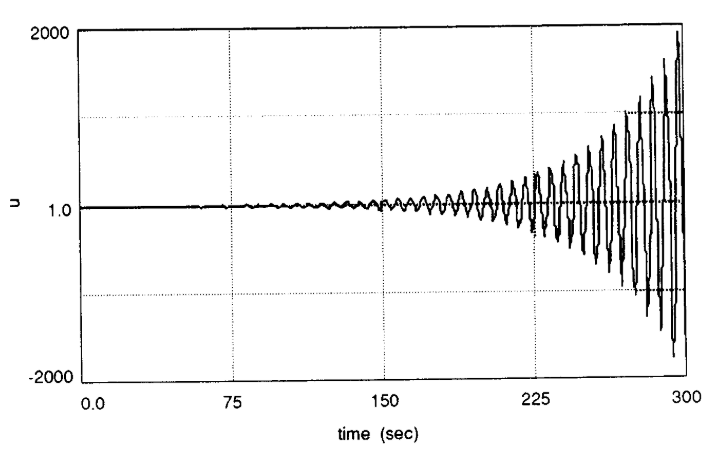
\includegraphics[scale=0.2]{img/nonmin.png}
	\caption{}
	\end{minipage} \hfill
	\begin{minipage}{0.45\textwidth}
	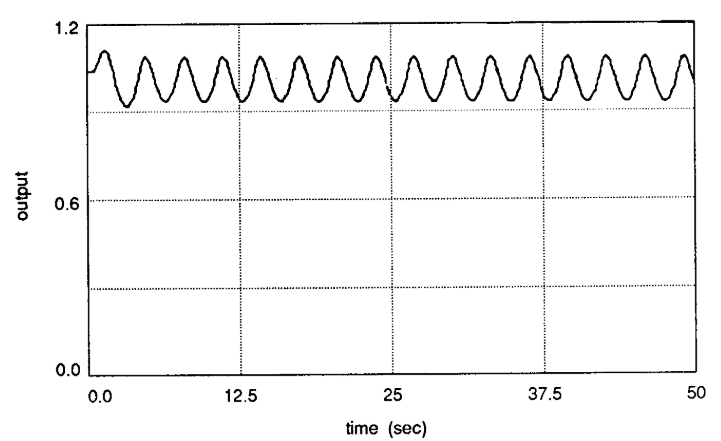
\includegraphics[scale=0.2]{img/nonmin2.png}
	\caption{}
	\end{minipage}
\end{figure} 
\end{frame}


\subsection{Field Overview}

\begin{frame}{Gain Scheduling Control Design}
    \begin{itemize}
        \item Nonlinear systems that can be covered by the LPV framework: hybrid dynamical systems, jump linear systems and switched linear systems. \autocite{Hoffmann2015}
        
        \item Algorithm:
        \begin{itemize}
            \item model
            \item design
            \item implementation
            \item performance assessment
        \end{itemize}
        
    \end{itemize}
\end{frame}


\begin{frame}{Field Overview - Modeling}
    \begin{itemize}
        \item Affine 
        \begin{equation}  \label{eq:poly_LPV}
\begin{bmatrix}
\dot{x}\\
y
\end{bmatrix} = \begin{pmatrix}\begin{bmatrix}
A_0 & B_0\\
C_0 & D_0
\end{bmatrix} + \sum_{i=1}^{N}\rho_i(t)\begin{bmatrix}
A_i & B_i\\
C_i & D_i
\end{bmatrix} \end{pmatrix} \begin{bmatrix}
x\\
u
\end{bmatrix}
\end{equation}
Polytopic LPV: if $A_0,B_0,C_0,D_0 = 0$, $\sum_{i=1}^{N}\rho_i(t) = 1, \displaystyle \rho_i(t) \geq 0$.
\item Linear Fractional Transformation
\begin{equation} \label{eq:LFT_upper}
\begin{bmatrix}
\dot{x}\\
z\\
y
\end{bmatrix} = \begin{bmatrix}
A(P)		&B_w(P) 	&B_u(P) \\
C_z(P) 	&D_{zw}(P) &D_{zu}(P)\\
C_y(P) 	&D_{yw}(P) &D_{yu}(P)
\end{bmatrix}\begin{bmatrix}
x\\
w\\
u
\end{bmatrix}
\end{equation}
with 
\begin{multline} \label{eq:LFT_theta}
\begin{bmatrix}
A(P)		&B_w(P) 	&B_u(P) \\
C_z(P) 	&D_{zw}(P) &D_{zu}(P)\\
C_y(P) 	&D_{yw}(P) &D_{yu}(P)
\end{bmatrix} = \begin{bmatrix}
A		&B_w 	&B_u\\
C_z 	&D_{zw} &D_{zu}\\
C_y 	&D_{yw} &D_{yu}
\end{bmatrix} + \\ \begin{bmatrix} 
B_p\\
D_{zp}\\
D_{yp}
\end{bmatrix}P(I-D_{lp}P)^{-1} \begin{bmatrix} C_l &D_{lw} &D_{lu}\end{bmatrix}
\end{multline}
    \end{itemize}
\end{frame}

\begin{frame}{Field Overview}
\begin{itemize}
        \item Importance of representation choice: system characteristics, feasibility of design problem
        
        \item Types of representation can be transformed between each one
        
        \item Modeling techniques: Jacobian linearization, State transformation, nonlinear embedding, etc. 

\end{itemize}
\end{frame}

\begin{frame}{Field Overview}
    \begin{itemize}
        \item Analysis: non minimum phase behavior, loss of stability, controllability and other characteristics
        
        \item Various blank spaces in the literature
    \end{itemize}
\end{frame}

\begin{frame}{Field Overview}
    \begin{itemize}
        \item Synthesis: Lyapunov based methods, Small gain theorem, Invariant set methods
        
        \item State feedback, output feedback and dynamic controllers
        
        \item Type of Lyapunov function: quadratic, polynomial, fuzzy, etc.
        
    \item The field mainly focuses on decreasing conservativeness and obtaining alternative forms of design
    \end{itemize}
\end{frame}

\begin{frame}{Field Overview}
    \begin{itemize}
        \item Computational issues: obtaining a tractable problem, with a finite number of constraints, convexity of the parameter space, etc.
        
        \item NP-hard problems, BMI problems, why are LMIs important
        
        \item Implementation issues: parameter measurement or estimation, controller causality, etc.
    \end{itemize}
\end{frame}
\subsection{What's lacking in literature}
\begin{frame}{What's lacking in literature}
       \begin{itemize}
        \item Updated survey and field overview
        \item Real applications and higher order systems
        \item Relationship between LPV and T-S Fuzzy
        \item Controllability of LPV systems
        % \item Obtaining LMIs from stability conditions
    \end{itemize}
\end{frame}


\section{LPV vs T-S Fuzzy}
\begin{frame}{LPV vs Takagi-Sugeno Fuzzy}
    \begin{itemize}
        \item There exists a close connection between the LPV and Takagi-Sugeno fuzzy frameworks \autocite{Rotondo2018} that has not been fully explored by the literature
    \end{itemize}
\end{frame}

\begin{frame}{A few citations}
    \begin{itemize}
        \item Control design for a mobile robot: a fuzzy LPV approach \autocite{Tsourdos}
        
        \item Flight Control Design For A STT Missile: A Fuzzy LPV Approach \autocite{Blumel2017}
        
        \item State-Feedback H$\infty$ Control for LPV System Using T-S Fuzzy Linearization Approach \autocite{Liu2013}
        
    \end{itemize}
\end{frame}

\begin{frame}{A few citations}
    \begin{itemize}
    \item Continuous quasi-LPV Systems: how to leave the quadratic Framework? \autocite{JAADARI2013}
        
    \item Automated generation and comparison of Takagi–Sugeno and polytopic quasi-LPV models \autocite{Rotondo2015}
    \end{itemize}
\end{frame}

\begin{frame}{Takagi-Sugeno Fuzzy systems}
    \begin{definition} A Linear Takagi-Sugeno  fuzzy model \autocite{Tanaka2001} is a representation of a nonlinear system, described by fuzzy IF-THEN rules of the form
\begin{equation} \label{tsfuzzysys}
\begin{array}{l}
\mbox{IF ~ } \big(z_1(t)\mbox{~is~} M_{i1}\big) \mbox{~and~} \big(z_2(t)\mbox{~is~} M_{i2}\big)\mbox{~and~} \ldots \mbox{~and~}\big(z_p(t) \mbox{~is~} M_{ip}\big
),\\[1mm]
\mbox{THEN~}
\left\{\begin{array}{l}
\dot{x}(t)={A}_i{x}(t) + B_iu(t),\\
y(t)={C}_i{x}(t),
\end{array} \right. \quad i=1,2,\ldots, r.
\end{array}    
\end{equation}
where $M_{ij}$ is the Fuzzy set, $r$ the number of model rules and $z_i(t)$ is the $i^{th}$ premise variable, which can either be a function of the states or external disturbances. 
\end{definition}
\end{frame}

\begin{frame}{Takagi-Sugeno Fuzzy systems}
    The overall fuzzy model of the system is achieved by fuzzy blending of the local models, that is, given a pair $(x(t),u(t))$, the final output is inferred as
\begin{eqnarray} \label{tsfuzzyblend}
    \dot{x} &=& \displaystyle  \sum_{i=1}^{r}h_i(z(t))\{A_ix(t)+B_iu(t)\}\\
y&=& \displaystyle  \sum_{i=1}^{r}h_i(z(t))C_ix(t)
\end{eqnarray}
where $h_i(z(t))$ are called the membership functions and satisfy the following convexity properties
\begin{equation}
    \displaystyle\sum_{i=1}^{r}h_i(z(t)) = 1, \displaystyle h_i(z(t)) \geq 0.
\end{equation}
\end{frame}

\begin{frame}{Automated generation and comparison of Takagi–Sugeno and polytopic quasi-LPV models \autocite{Rotondo2015}}
\begin{table}[htb]
    \centering
    \renewcommand{\arraystretch}{1.5}
    \begin{tabularx}{\textwidth}{
    |>{\centering\arraybackslash}X 
    |>{\centering\arraybackslash}X | }
    \hline Polytopic LPV & T-S fuzzy\\ \hline \hline
    $\sigma.x(\tau) = \displaystyle  \sum_{i=1}^{N}\pi_i(\theta(\tau))(A_ix(\tau)+B_iu(\tau))$ & $\sigma.x(\tau) = \displaystyle  \sum_{i=1}^{N}\omega_i(\nu(\tau))(A_ix(\tau)+B_iu(\tau))$\\
    $y= \displaystyle \sum_{i=1}^{N}\pi_i(\theta(\tau))C_ix(\tau)$ &
    $ y= \displaystyle  \sum_{i=1}^{N}\omega_i(\nu(\tau))C_ix(t)$ \\
    $\displaystyle\sum_{i=1}^{N}\pi_i(\theta(\tau)) = 1$ &
    $\displaystyle\sum_{i=1}^{N}\omega_i(\nu(\tau)) = 1$ \\
    $\displaystyle \pi_i(\theta(\tau)) \geq 0$ &
    $\displaystyle \omega_i(\nu(\tau)) \geq 0$ \\
    \hline
    \end{tabularx}
    \label{tab:comp}
\end{table}
\end{frame}

\begin{frame}{Automated generation and comparison of Takagi–Sugeno and polytopic quasi-LPV models}
Problems:
    \begin{itemize}
        \item LPV notation is not standard, hindering a more profound analysis
        \item Sector nonlinearity application
    \end{itemize}
\end{frame}
\begin{frame}{Our proposal}
    The equivalence between T-S fuzzy and LPV goes beyond what is stated in Rotondo et al.
    \begin{table}[htb]
    \centering
    \begin{tabularx}{\textwidth}{c|c}
         Polytopic LPV& T-S fuzzy  \\ \hline \hline
                $ \dot{x} = \displaystyle  \sum_{i=1}^{N}\rho_i(t)\{A_ix(t)+B_iu(t)\}$ & $\dot{x} = \displaystyle  \sum_{i=1}^{r}h_i(z(t))\{A_ix(t)+B_iu(t)\}$ \\
                $y= \displaystyle \sum_{i=1}^{N}\rho_i(t)C_ix(t)$ &  $ y= \displaystyle  \sum_{i=1}^{r}h_i(z(t))C_ix(t)$ \\
                $\displaystyle\sum_{i=1}^{N}\rho_i(t) = 1$ & $\displaystyle\sum_{i=1}^{r}h_i(z(t)) = 1$ \\
                $\displaystyle\rho_i(t) \geq 0$ & $\displaystyle h_i(z(t)) \geq 0$
     \end{tabularx}
    \label{tab:mycomp}
\end{table}
\end{frame}

\begin{frame}{Our proposal}
\begin{itemize}
        \item T-S fuzzy is a special case of LPV systems
        \item Polytopic LPV and T-S fuzzy are indistinguishable for control design. 
        % \item Proof: 
        % \begin{itemize}
        %     \item formal definition of LPV systems (not found in literature)
        %     \item every polytopic LPV system can be approximated by a T-S fuzzy model
        % \end{itemize}
    \end{itemize}
\end{frame}
\begin{frame}{}
    \begin{theorem}
A T-S fuzzy system is a polytopic LPV system.
\end{theorem}
\begin{proof} \renewcommand{\qedsymbol}{}
To prove this affirmation, we will write the T-S fuzzy system \eqref{tsfuzzyblend} in the form of \eqref{eq:poly_LPV}. First, we write it in vector form
\begin{equation} \label{fuzzy_lpv}
 \begin{bmatrix}
    \dot{x}\\
    y
 \end{bmatrix} = \begin{bmatrix} 
\displaystyle    \sum_{i=1}^{r}h_i(z(t))A_i & \displaystyle \sum_{i=1}^{r}h_i(z(t))B_i\\
\displaystyle    \sum_{i=1}^{r}h_i(z(t))C_i & 0
 \end{bmatrix}\begin{bmatrix}
 x\\
 u
 \end{bmatrix}.
\end{equation}
Then, choose
\begin{equation}
    \rho_i(t) :=  h_i(z(t)) ~~\forall i \in \{1,...,r\}
\end{equation}
\end{proof}
\end{frame}

\begin{frame}{}
    \begin{proof}
So we can write
\begin{eqnarray} \label{matrices}
\sum_{i=1}^{r}\rho_i(t)A_i =  \sum_{i=1}^{r}h_i(z(t))A_i\\
\sum_{i=1}^{r}\rho_i(t)B_i =  \sum_{i=1}^{r}h_i(z(t))B_i\\
\sum_{i=1}^{r}\rho_i(t)C_i =  \sum_{i=1}^{r}h_i(z(t))C_i
\end{eqnarray}
Substituting these into \eqref{fuzzy_lpv} yields \eqref{eq:poly_LPV}, thus completing the proof. 
\end{proof}
\end{frame}

\begin{frame}{Next Steps}
    \begin{itemize}
        \item Even though this proof is simple, it has not been done before.
        \item We are working on proving that any LPV system can be represented by a T-S fuzzy system 
        \item Further analyze the implications of the relationship between them
    \end{itemize}
\end{frame}

% \begin{frame}{Automated generation and comparison of Takagi–Sugeno and polytopic quasi-LPV models}
% \blockquote{There are strong analogies between polytopic LPV and TS systems. In fact, the only remarkable difference between
% the two frameworks is the set of mathematical tools that are used for obtaining the system description. In the LPV case, these tools belong to the standard mathematics; on the other hand, in the TS case, they belong to the fuzzy theory. In particular, the correspondences between polytopic LPV and TS systems are between:
% \begin{itemize}
%     \item the scheduling parameters $\theta$ of LPV systems and the premise variable $\nu$ of TS systems; 
%     \item the coefficients of the polytopic decomposition $\pi_i$ and the coefficients $\rho_i$ that describe the level of activation of each local model;
% \item the vertex systems in the polytopic LPV case and the subsystems in the TS case
% \end{itemize}}
% \end{frame}


% \begin{frame}
% 	Idea: prove that a general polytopic LPV system satisfies the assumptions and, therefore, can be approximated by a T-S model. 
	
% 	(??) Can the corollary be applied?
	
% 	\begin{eqnarray} 
%     \dot{x} &=& \displaystyle  \sum_{i=1}^{N}\rho_i\{A_ix(t)+B_iu(t)\}\\
% y&=& \displaystyle  \sum_{i=1}^{N}\rho_iC_ix(t)\\
% && \displaystyle\sum_{i=1}^{N}\rho_i = 1, \displaystyle \rho_i \geq 0.
% \end{eqnarray}

% \end{frame}

% \section{Formal definition of LPV systems}
% \begin{frame}{Definition of LPV systems}
% The definition we wish to propose should be
% \begin{itemize}
%         \item A special case of a definition of a dynamic system
%         \item The general representation should be $\dot{x} = A(\rho)x+B(\rho)u$
%         \item Needs to be valid for affine and LFT parameter dependencies
%     \end{itemize}
% \end{frame}

% \begin{frame}{Definition of dynamical system}
% A continuous-time dynamical system $\mathcal{G}$ is the octuple $(\mathcal{D,U},U,\mathcal{Y},Y,\mathbb{R},s,h)$, where $s: \mathbb{R} \times \mathbb{R} \times \mathcal{D} \times \mathcal{U} \rightarrow \mathcal{D}$ and $h: \mathbb{R} \times \mathcal{D} \times U \rightarrow Y$ are such that the following axioms hold \autocite{Chellaboina2008}:

% \begin{itemize}
%     \item(Continuity) For every $t_0 \in \mathbb{R}, x_0 \in \mathcal{D}$ and $u \in \mathcal{U}, s(.,t_0,x_0,u)$ is continuous for all $t \in \mathbb{R}$ and continuously differentiable on $\mathcal{D}$ 
%     \item(Consistency) For every $x_0 \in \mathcal{D}, u \in \mathcal{U}$, and $t_0 \in \mathbb{R}, ~s(t_0,t_0,x_0,u) = x_0$
%     \item(Determinism) For every $t_0 \in \mathbb{R}$ and $x_0 \in \mathcal{D}, ~s(t,t_0,x_0,u_1) = s(t,t_0,x_0,u_2)$ for all $t \in \mathbb{R}$ and $u_1,u_2 \in \mathcal{U}$ satisfying $u_1(\tau) = u_2(\tau), \tau \in [t_0,t]$
% \end{itemize}
% \end{frame}

% \begin{frame}{Definition of dynamical system}
% \begin{itemize}
%     \item(Group property) $s(t_2,t_0,x_0,u) = s(t_2,t_1,s(t_1,t_0,x_0,u),u)$ for all $t_0,t_1,t_2 \in \mathbb{R}, t_0 \leq t_1 \leq t_2, x_0 \in \mathcal{D}$, and $u \in \mathcal{U}$.
%     \item(Read-out map) There exists $y \in \mathcal{Y}$ such that $y(t) = h(t,s(t,t_0,x_0,u),u(t))$ for all $x_0 \in \mathcal{D}, u \in \mathcal{U}, t_0 \in \mathbb{R}$, and $t \in \mathbb{R}$.
% \end{itemize}
% The map $s(t,t_0,x_0,u)$ is referred to as the flow or trajectory of the dynamical system and choosing $x(t) = s(t,t_0,x_0,u)$ it gives rise to a differential equation of the form
% \begin{equation}
%     \dot{x} = F(t,x,u), \quad x(t_0) = x_0, \quad t \geq t_0
% \end{equation}
% where
% \begin{equation}
% F(t,x,u) = \frac{dx}{dt} = \frac{\partial s}{\partial t}(t,t_0,x,u) \bigg|_{t=t_0}.     
% \end{equation}
% We represent dynamical systems through their differential equation \hfill $\triangle$
% \end{frame}

% \begin{frame}{Definition of LPV system}
% An LPV system is a continuous-time dynamical system 
% nonuple $(\mathcal{D,P, U},U,\mathcal{Y},Y,\mathbb{R},s,h)$, where $s: \mathbb{R} \times \mathbb{R} \times \mathcal{D} \times \mathcal{P} \times \mathcal{U} \rightarrow \mathcal{D}$ and $h: \mathbb{R} \times \mathcal{D} \times U \rightarrow Y$ 
% such that the following axioms hold:
% \begin{itemize}
%     \item it is a continuous-time dynamical system
%     \item (Additivity) $s(t,t_0,x_1,\rho,u_1) + s(t,t_0,x_2,\rho,u_2) = s(t,t_0,x_1+x_2,\rho,u_1+u_2)$
%     \item (Homogeneity) $s(t,t_0,\alpha x_0,\rho,\alpha u) = \alpha s(t,t_0,x_0,\rho,u)$
%     \item $\rho = \rho(t) \in \mathcal{P}$
% \end{itemize}
% \end{frame}

% \begin{frame}{Definition of LPV system}
%     If we choose s as 
% \begin{equation}
%     s(t,t_0,x_0,\rho,u) = \Phi(t,t_0)x_0 + \int_{t_0}^t\Phi(t,\tau)B(\rho)u(\tau)d\tau
% \end{equation}
% where $\Phi(t,t_0)$ denotes the state transition matrix given by the Peano-Baker series \autocite{Antsaklis2006}
% \begin{equation}
%     \Phi(t,t_0) = I + \int_{t_0}^tA(\rho(\tau_1))d\tau_1 + \int_{t_0}^tA(\rho(\tau_1))\int_{t_0}^{\tau_1}A(\rho(\tau_2))d\tau_2d\tau_1 + ...
% \end{equation}
% \end{frame}

% \begin{frame}{Definition of LPV system}
%     Lets derive the ODE form
% \begin{gather*}
%     \frac{ds}{dt}(t,t_0,x,\rho,u) = \dot{\Phi}(t,t_0)x + \Phi(t,t)B(\rho)u\cdot1 - \Phi(t,t_0)B(\rho)u\cdot0 + \\ \int_{t_0}^t\dot{\Phi}(t,\tau)B(\rho)ud\tau\\
%     \frac{ds}{dt}(t,t_0,x,\rho,u) = A(\rho)\Phi(t,t_0)x + \Phi(t,t)B(\rho)u + \int_{t_0}^tA(\rho)\Phi(t,\tau)B(\rho)ud\tau\\
%     \frac{ds}{dt}(t,t_0,x,\rho,u) \bigg|_{t=t_0} = A(\rho)\Phi(t,t_0)x + \Phi(t,t)B(\rho)u(t) +\\ \int_{t_0}^tA(\rho)\Phi(t,\tau)B(\rho)u(\tau)d\tau \\
%     \Rightarrow \dot{x}(t) = A(\rho)x(t) + B(\rho)u(t), \quad x(t_0) = x_0, \quad t \geq t_0
% \end{gather*}
% \end{frame}

% \begin{frame}{Definition of LPV system}
%     the ODE derived from $s$ has the general form
% \[\dot{x} = A(\rho(t))x+B(\rho(t))u\]
% where $x(t) \in \mathbb{R}^n$ is the state vector, $u(t) \in \mathbb{R}^{n_i}$ is the input vector,   $\rho(t) \in \mathbb{R}^N$ is the vector of time-varying parameters, also called scheduling parameters, and $A$ and $B$ are matrices of appropriate dimensions. The scheduling parameters can be a function of time, state, input, external parameter or any combination of those.
% \end{frame}

% \begin{frame}{Summary}
% Advantages of the LPV - Fuzzy "merge"
% \begin{itemize}
%     \item Major fields developed independently, results can be exchanged
%     \item Use of sector nonlinearity
%     \item T-S fuzzy non quadratic framework
% \end{itemize}
% \end{frame}
% \section{PhD Project}
% \begin{frame}{PhD Project}
%     Results so far:
% \begin{itemize}
%     \item Comprehensive literature/field review
%     \item Formally defined LPV systems
%     \item Proved that T-S fuzzy is a special case of LPV systems
%     \item 4 different models of a real quadrotor
%     \item Designed and applied controller to quadrotor (experimental and simulation results)
%     \item Controllability results: we were not able to find feasible output feedback controllers for any of the models. Few, contradictory results in the literature.
%     \item Generalized control energy (model with unique equilibrium at the origin)
%     \item SBAI
%     \item DINCON
%     \item ICUAS
% \end{itemize}
% \end{frame}

% \begin{frame}{Timeline}
%     \begin{itemize}
%     \item End of scholarship: July 30th
%     \item Presentation: July or August
%     \item Final results: March
% \end{itemize}
% \end{frame}

% \begin{frame}{Next steps}
%     \begin{itemize}
%     \item Prove that T-S fuzzy theorems work for polytopic LPV
%     \item Submit a journal paper*
%     \item Comments: modeling uncertainty in real life applications
% \end{itemize}
% \end{frame}
% %%%%%%%%%%%%%%%%%%%%%%%%%%%%%%%% FRAME %%%%%%%%%%%%%%%%%%%%%%%%%%%%%%%%

% % \begin{frame}{Modeling}{Linear Fractional Representation vs Affine}
% % 			\begin{figure} 
% % 				\centering
% % 				\begin{tikzpicture}[node distance=1cm, auto]  
% % 				\tikzset{
% % 					mynode/.style={rectangle,rounded corners,draw=black, top color=white, bottom color=blue!30,very thick, inner sep=1em, minimum size=4em, text centered},
% % 					mynode2/.style={rectangle,rounded corners,draw=black, top color=white, bottom color=blue!30,very thick, inner sep=1em, minimum size=6em, text centered},
% % 					myarrow/.style={->, >=latex', shorten >=1pt, thick},
% % 					mylabel/.style={text width=7em, text centered} 
% % 				}  
% % 				\node[mynode] (manufacturer) {${\rho}(k)$};  
% % 				\node[below=3cm of manufacturer] (dummy) {}; 
% % 				\node[mynode2, below=0.3cm of manufacturer] (retailer1) {${M}$};  
% % 				% The text width of 7em forces the text to break into two lines. 
				
% % 				% \draw[myarrow] (retailer1.west) -- ++(-.5,0) -|  (manufacturer.west);	
% % 				\draw[myarrow] (-1.25,-1.55)-- ++(-.5,0) -- ++(0,+1.6) -- ++(0.96,0);	
% % 				\draw[myarrow] (0.84,0) -- ++(.95,0) -- ++(0,-1.6) -- ++(-0.57,0);
				
% % 				\node at (-1.7,0.35) {$l(k)$};
% % 				\node at (+1.7,0.35) {$p(k)$};
				
% % 				% There is a slight overlap of the arrows with the (manufacturer) south edge
% % 				% because creating the offset in another way didn't compile. 
				
% % 				\draw[myarrow] (-1.05-0.2,-2.15-0.56) + (0,0.6)-- ++(-1,0.6);
% % 				\draw[myarrow] (-1.05-0.2,-2.15-1.12) + (0,0.6)-- ++(-1,0.6);
% % 				\draw[myarrow] (-1.05-0.2,-3.35-0.5) + (0,0.6)-- ++(-1,0.6);
				
				
				
% % 				\node at (-2.85-0.2,-2.1) {$x(k+1)$};
% % 				\node at (-2.55-0.2,-2.1-0.56) {$z(k)$};
% % 				\node at (-2.55-0.2,-2.1-1.12) {$y(k)$};
				
				
% % 				\draw[myarrow] (+2.03+0.18,-2.15-0.56)+ (0,0.6)-- ++(-1,0.6);
% % 				\draw[myarrow] (+2.03+0.18,-2.15-1.12)+ (0,0.6)-- ++(-1,0.6);
% % 				\draw[myarrow] (+2.03+0.18,-3.35-0.5)+ (0,0.6)-- ++(-1,0.6);
				
% % 				\node at (+2.6+0.18,-2.1) {$x(k)$};
% % 				\node at (+2.6+0.18,-2.1-0.56) {$w(k)$};
% % 				\node at (+2.6+0.18,-2.1-1.12) {$u(k)$};
				
% % 				% \draw[<->, >=latex', shorten >=2pt, shorten <=2pt, bend right=45, thick, dashed] 
% % 				%     (retailer1.south) to node[auto, swap] {Competition}(retailer2.south); 
% % 				% The swap command corrects the placement of the text.
				
% % 				\end{tikzpicture} 
% % %				\medskip
% % %				\caption{LFT plant diagram} \label{fig:LFTdiagram}
% % 			\end{figure}
% % 			\vspace{-0.5cm}
% % 			\begin{equation*} 
% % 			\begin{bmatrix}
% % 			l \\ \hline
% % 			\dot{x}\\
% % 			z\\
% % 			y
% % 			\end{bmatrix} = \begin{bmatrix} \begin{array}{c|ccc}
% % 			D_{lp}  &C_l 	&D_{lw} &D_{lu}\\
% % 			\hline
% % 			B_p		&A		&B_w 	&B_u \\
% % 			D_{zp}	&C_z 	&D_{zw} &D_{zu}\\
% % 			D_{yp}	&C_y 	&D_{yw} &D_{yu}
% % 			\end{array} \end{bmatrix}\begin{bmatrix}
% % 			p\\ \hline
% % 			x\\
% % 			w\\
% % 			u
% % 			\end{bmatrix}, ~p = P l
% % 			\end{equation*}		
	
% % \end{frame}

% %%%%%%%%%%%%%%%%%%%%%%%%%%%%%%%% FRAME %%%%%%%%%%%%%%%%%%%%%%%%%%%%%%%%

% % \begin{frame}{Modeling}{Linear Fractional Representation vs Affine}
% % \begin{equation*} \label{eq:LFT_upper}
% % \begin{bmatrix}
% % \dot{x}\\
% % z\\
% % y
% % \end{bmatrix} = \underbrace{\begin{bmatrix}
% % A(P)		&B_w(P) 	&B_u(P) \\
% % C_z(P) 	&D_{zw}(P) &D_{zu}(P)\\
% % C_y(P) 	&D_{yw}(P) &D_{yu}(P)
% % \end{bmatrix}}\begin{bmatrix}
% % x\\
% % w\\
% % u
% % \end{bmatrix}
% % \end{equation*}

% % \begin{equation*} 
% %  \begin{bmatrix}
% % A		&B_w 	&B_u\\
% % C_z 	&D_{zw} &D_{zu}\\
% % C_y 	&D_{yw} &D_{yu}
% % \end{bmatrix} + \begin{bmatrix} 
% % B_p\\
% % D_{zp}\\
% % D_{yp}
% % \end{bmatrix}P(I-D_{lp}P)^{-1} \begin{bmatrix} C_l &D_{lw} &D_{lu}\end{bmatrix}
% % \end{equation*}

% % \end{frame}

% %%%%%%%%%%%%%%%%%%%%%%%%%%%%%%%% FRAME %%%%%%%%%%%%%%%%%%%%%%%%%%%%%%%%

% % \begin{frame}{Modeling}{Affine Parameter Dependency}
% % \begin{itemize}
% % 	\item Importance of the type of representation
% % \end{itemize}
% % \vspace{1cm}
% % An LPV system is said to have affine parameter dependency if it can be represented by 
% % \begin{equation}  
% % \begin{bmatrix}
% % \dot{x}\\
% % y
% % \end{bmatrix} = \begin{pmatrix}\begin{bmatrix}
% % A_0 & B_0\\
% % C_0 & D_0
% % \end{bmatrix} + \sum_{i=1}^{N}\rho_i(t)\begin{bmatrix}
% % A_i & B_i\\
% % C_i & D_i
% % \end{bmatrix} \end{pmatrix} \begin{bmatrix}
% % x\\
% % u
% % \end{bmatrix}
% % \end{equation}
% % \end{frame}

% %%%%%%%%%%%%%%%%%%%%%%%%%%%%%%%% FRAME %%%%%%%%%%%%%%%%%%%%%%%%%%%%%%%%

% % \begin{frame}{Modeling}{Affine Parameter Dependency}
% %     \begin{itemize}
% % 	\item [--] Overboundedness problem
% % 	\item [+] Combined with Lyapunov theory, naturally derives LMI based design conditions
% % 	\item Modeling procedures: Jacobian linearization, state transformation, nonlinear embedding, TS-fuzzy, etc.
	
% % \end{itemize}
% % \end{frame}
% % \begin{frame}{Modeling}{Affine LPV Systems}
% % \begin{itemize}
% % 	\item Importance of the type of representation
% % % 	\item Focus on affine
% % 	\item Modeling procedures: Jacobian linearization, state transformation, nonlinear embedding, TS-fuzzy, etc.
% % \end{itemize}
	
% % \end{frame}
% %%%%%%%%%%%%%%%%%%%%%%%%%%%%%%%% FRAME %%%%%%%%%%%%%%%%%%%%%%%%%%%%%%%%

% % \begin{frame}{Takagi-Sugeno fuzzy systems}
% % \begin{block}{Definiton}
% % A Takagi-Sugeno  fuzzy model is a representation of a dynamical nonlinear system, described by fuzzy IF-THEN rules of the form \autocite{Tanaka2001}
% % \begin{equation}
% % \begin{array}{l}
% % \mbox{If ~ } \big(z_1(t)\mbox{~is~} M_{i1}\big) \mbox{~and~} \big(z_2(t)\mbox{~is~} M_{i2}\big)\mbox{~and~} \ldots \mbox{~and~}\big(z_p(t) \mbox{~is~} M_{ip}\big
% % ),\\[1mm]
% % \mbox{then~}
% % \left\{\begin{array}{l}
% % \dot{x}(t)={A}_i{x}(t)+{B}_i{u}(t),\\
% % y(t)={C}_i{x}(t),
% % \end{array} \right. \quad i=1,2,\ldots, r.
% % \end{array}    
% % \end{equation}
% % where $M_{ij}$ Fuzzy set, $r$ number of model rules, $z_i(t)$ $i^{th}$ premise variable, $x \in \mathbb{R}^{n}$ state vector, $u \in \mathbb{R}^{n}$ input vector, $y \in \mathbb{R}^{n}$ output vector, $A, B$ and $C$ matrices of appropriate dimensions. 
% % \end{block}


% % \end{frame}

% %%%%%%%%%%%%%%%%%%%%%%%%%%%%%%%% FRAME %%%%%%%%%%%%%%%%%%%%%%%%%%%%%%%%

% % \begin{frame}{Takagi-Sugeno fuzzy systems}
% % 	Similarities between polytopic LPV and TS-fuzzy \autocite{Rotondo2016}:
% % 	\begin{itemize}
% % 		\item Membership functions work as scheduling parameters 
% % 		\item Local models correspond to vertex systems
% % 		 \item They have been treated as different by the research community and therefore researched independently. However, a few recent publications have been exploring the similarities.
% % 	\end{itemize}
% % \end{frame}

% %%%%%%%%%%%%%%%%%%%%%%%%%%%%%%%% FRAME %%%%%%%%%%%%%%%%%%%%%%%%%%%%%%%%
% % 11111

% % \begin{frame}{LPV Analysis and Synthesis}
% % 	Consider the general autonomous LPV system
% % 	\begin{equation} 
% % 	\dot{x} = A(\rho)x \label{eq:aut_LPV}
% % 	\end{equation}
% % 	where $\rho \in P \subset \mathbb{R}^N$. Initally, we do not restrict the form of $A(\rho)$ or $P$. The most intuitive, simple Lyapunov function candidate and, usually, the first to be tested is the quadratic
% % 	\begin{equation}
% % 	V(x) = x^TPx
% % 	\end{equation}
% % 	where $P^T=P > 0$ is not a function of the varying parameter. Taking its time derivative yields
% % 	\begin{equation}
% % 	\dot{V}(x) = x^T(A^T(\rho)P + PA(\rho))x
% % 	\end{equation}
% % 	which results in the following stability condition
% % 	\begin{equation} 
% % 	A^T(\rho)P + PA(\rho) < 0, \forall ~\rho(t) \in P. \label{eq:stab}
% % 	\end{equation}
% % \end{frame}

% %%%%%%%%%%%%%%%%%%%%%%%%%%%%%%%% FRAME %%%%%%%%%%%%%%%%%%%%%%%%%%%%%%%%
% % \begin{frame}{LPV Analysis and Synthesis}
% % 	\begin{itemize}
% % 		\item Has to be solved numerically
% % 		\item Infinite dimensional
% % 		\item Infinite constraints
% % 	\end{itemize}
	
% % 	\begin{block}{}
% % 		At some point the study of LPV analysis and synthesis becomes the study of turning a infinitely constrained infinite dimensional problem into a tractable one with a finite number of constraints that must give the same stability and performance properties. Furthermore, the problem needs to be in a form that is compatible with the currently available solvers.  
% % 	\end{block}
% % \end{frame}

% % \begin{frame}{LPV Analysis and Synthesis}
% % In order to do this, a number of assumptions is usually made:
% % \begin{itemize}
% % 	\item Plant description (model in one of the forms discussed earlier);
% % 	\item Convexity of the parameter set;
% % 	\item Form of the controller (state feedback \autocite{Rotondo2016}, output feedback \autocite{Al-Jiboory2018} and dynamic controllers \autocite{Veenman2014});
% % 	\item Form of the Lyapunov function (quadratic, polynomial and affine),
% % \end{itemize}
% % \end{frame} 
% % \begin{frame}{LPV Analysis and Synthesis}
% % 	Frequently, the chosen numerically tractable forms are LMIs because they can be globally and efficiently solved by interior point methods in semidefinite programming \autocite{Tuan2001}.
% % \end{frame}
% %%%%%%%%%%%%%%%%%%%%%%%%%%%%%%%% FRAME %%%%%%%%%%%%%%%%%%%%%%%%%%%%%%%%



% % \begin{frame}{Synthesis Techniques}
% % 	\begin{itemize}
% % 		\item Small-gain Theorem
% % 		\item Lyapunov Theory: quadratic and non-quadratic
% % 		\item Invariant Set Theory
% % 	\end{itemize}
	
% % \end{frame}

% %%%%%%%%%%%%%%%%%%%%%%%%%%%%%%%% FRAME %%%%%%%%%%%%%%%%%%%%%%%%%%%%%%%%
% %\begin{frame}{Research topics}{Affine LPV Systems}
% %	\begin{itemize}
% %		\item Modeling
% %		\item Similarities between polytopic LPV and TS-fuzzy
% %		\item Reducing conservatism of design conditions: using alternative Lyapunov functions, introduction of slack variables, invariant set techniques, etc
% %	\end{itemize}
% %	
% %\end{frame}


% %%%%%%%%%%%%%%%%%%%%%%%%%%%%%%%% FRAME %%%%%%%%%%%%%%%%%%%%%%%%%%%%%%%%

% % \begin{frame}{Lyapunov Theory}
% % 	Consider the following polytopic LPV system 
% % 	\begin{eqnarray} \label{eq:syn_sys}
% % 	\dot{x} = \sum_{i=1}^{N}\rho_i(t)A_i x + Bu.
% % 	%y = \sum_{i=1}^{N}\rho_i(t)C_i x + \sum_{i=1}^{N}\rho_i(t)D_i u
% % 	\end{eqnarray}
% % 	For a quadratic Lyapunov function 
% % 	\begin{equation} \label{eq:quad_lyap}
% % 	V(x) = x^TPx
% % 	\end{equation}
% % 	We have 
% % 	\begin{equation}
% % 	\dot{V}(x) = x^T\Big\{(\sum_{i=1}^{N}\rho_i(t)A^T_i + K^T_iB^T) P + P(\sum_{i=1}^{N}\rho_i(t)A_i + K_iB)\Big\}.
% % 	\end{equation}
% % 	Imposing negative definiteness and applying a change of variables, we can state the next theorem.
% % \end{frame}
% %%%%%%%%%%%%%%%%%%%%%%%%%%%%%%%% FRAME %%%%%%%%%%%%%%%%%%%%%%%%%%%%%%%%

% % \begin{frame}{Lyapunov Theory}
	
% % 		\begin{theorem}[Quadratic Stability]\autocite{Rotondo2016}
% % 			Let $Q > O$ and $\Gamma_i \in \mathbb{R}^{nxn}, i = 1, . . . ,N$ be such that:
% % 			\[
% % 			He\{A_iQ + B\Gamma_i\} < O  ~\forall i = 1, . . . ,N
% % 			\]
% % 			Then, the closed-loop system 
% % 			\begin{eqnarray} \label{eq:syn_sys}
% % 			\dot{x} = \sum_{i=1}^{N}\rho_i(t)A_i x + Bu.
% % 			%y = \sum_{i=1}^{N}\rho_i(t)C_i x + \sum_{i=1}^{N}\rho_i(t)D_i u
% % 			\end{eqnarray}
% % 			with $u= - \sum_{i=1}^{N}\rho_i(t)K_i x $ and gains calculated as $K_i = \Gamma_iQ^{-1}, i = 1, . . . ,N$ and $P = Q^{-1}$, is quadratically stable.
% % 		\end{theorem} 
% % \end{frame}
% %%%%%%%%%%%%%%%%%%%%%%%%%%%%%%%% FRAME %%%%%%%%%%%%%%%%%%%%%%%%%%%%%%%%

% % \begin{frame}{Lyapunov Theory}{Quadratic Stability}
	
% % 	\begin{itemize}
% % 		\item[--] Very conservative 
% % 		\item[+] Guarantees stability for arbitrarily fast parameter trajectories
% % 		\item Numerous results\autocite{Rotondo2016} based on quadratic stability with performance requirements 
% % 	\end{itemize}
	
% % \end{frame}%%%%%%%%%%%%%%%%%%%%%%%%%%%%%%%% FRAME %%%%%%%%%%%%%%%%%%%%%%%%%%%%%%%%

% % \begin{frame}{Lyapunov Theory}{Non-quadratic}
% % 	\begin{itemize}
% % 		\item  Reducing conservatism and exploring different forms of obtaining design conditions are the main active research areas for LPV and TS-fuzzy systems \autocite{JAADARI2013}$^{,}$\autocite{Guerra2009}
% % 		\item Alternative Lyapunov functions: affine parameter, polynomial, piecewise, etc
% % 	\end{itemize}
% % \end{frame}%%%%%%%%%%%%%%%%%%%%%%%%%%%%%%%% FRAME %%%%%%%%%%%%%%%%%%%%%%%%%%%%%%%%

% % \begin{frame}{Obtaining Synthesis Conditions}{Affine Parameter-dependent Lyapunov, a.k.a Fuzzy Lyapunov}
% % 	Consider the following closed loop system
% % 	\begin{equation} \label{eq22}
% % 	\dot e(t) = \sum_{i=1}^{r}\sum_{j=1}^{r}h_ih_j(A_{ij}-BK_i)e,
% % 	\end{equation}
% % 	and the following Lyapunov function candidate $V({e}(t)):S \rightarrow \mathbb{R}$:
% % 	\begin{equation}
% % 	\label{lyap}
% % 	V({e}(t))=\sum_{i=1}^{r}h_i{e}(t)'{P}_i{e}(t)
% % 	\end{equation}
% % 	where $S$ is a subset of $\mathbb{R}^N$.
	
% % \end{frame}
% %%%%%%%%%%%%%%%%%%%%%%%%%%%%%%%% FRAME %%%%%%%%%%%%%%%%%%%%%%%%%%%%%%%%
% % \begin{frame}{Obtaining Synthesis Conditions}{Affine Parameter-dependent Lyapunov, a.k.a Fuzzy Lyapunov}
% % 	As a consequence, the derivative of (\ref{lyap}) is given by
% % 	\begin{equation}
% % 	\label{der}
% % 	\dot V({e}(t))=\sum_{i=1}^{r}h_i\Bigl(
% % 	{\dot{e}}(t)' {P}_i{ e}(t) +{ e}(t)'{ P}_i{ \dot{e}}(t) \Bigr)+\sum_{\rho=1}^{r}\dot{h}_\rho{e}(t)'{P}_\rho{e}(t).
% % 	\end{equation}
% % 	The first-order time-derivative of the membership function $h_{i}$ appears in $\dot V({e}(t))$. By properties of the membership functions, it follows that
% % 	\[
% % 	\sum_{i=1}^{r}h_i=1 \Rightarrow \sum_{i=1}^{r}\dot h_i=0.
% % 	\]
% % 	Thus, \eqref{der} is nonconvex.
% % \end{frame}
% %%%%%%%%%%%%%%%%%%%%%%%%%%%%%%%% FRAME %%%%%%%%%%%%%%%%%%%%%%%%%%%%%%%%
% % \begin{frame}{Obtaining Synthesis Conditions}{Affine Parameter-dependent Lyapunov, a.k.a Fuzzy Lyapunov}
% %     \begin{itemize}
% %         \item The nonconvex term in \eqref{der}
% %         \item Several Results \autocite{Elias}$^{,}$\autocite{Mozelli2009}
% %     \end{itemize}
% % \end{frame}
% % \begin{frame}
% % 	Let us define the following set
% % 	\begin{equation}
% % 	\label{eqfi}
% % 	\mathcal{D}=\left\{e(t)\in S:|\dot{h}_{i}|\leq \phi_{i},~~\forall i\in \mathcal{R}\right\}
% % 	\end{equation}
% % 	where $\mathcal{R}=\{1,...,r\}$ and $\phi_{i}$ are given positive real numbers. 
% % 	\begin{lemma} \label{lema1}
% % 		\autocite{Tuan2001}Let be $\Psi_{ij}$ matrices of proper dimensions. If the following conditions hold 
% % 		\begin{align*}
% % 		\Psi_{ii}\prec {\bf 0},&\quad \forall i\in \mathcal{R},\\
% % 		\frac{1}{r-1}\Psi_{ii}+\Psi_{ij}+\Psi_{ji}\prec {\bf 0},&\quad \forall i,j\in \mathcal{R}, i<j,    
% % 		\end{align*}
% % 		then,
% % 		\[
% % 		\sum_{i=1}^{r}\sum_{j=1}^{r}h_ih_j\Psi_{ij}\prec {\bf 0}.
% % 		\]
		
	
% % 	\end{lemma}
% % \end{frame}
% %%%%%%%%%%%%%%%%%%%%%%%%%%%%%%%% FRAME %%%%%%%%%%%%%%%%%%%%%%%%%%%%%%%%
% % \begin{frame}
% % 		\begin{theorem}
% % 			\autocite{Mozelli2009}Let $\phi_{\rho}$ known positive real numbers satisfying \eqref{eqfi}. If, for a positive constant $\mu$, there exist matrices $\mathbf{ Z}\in \mathbb{R}^{N\times N}$, $\mathbf{ Y}_{i}\in \mathbb{R}^{r\times N}$, $\mathbf{X}=\mathbf{X}'\in \mathbb{R}^{N\times N}$ and $\mathbf{Q}_{i}=\mathbf{Q}_{i}'\in \mathbb{R}^{N\times N}$ satisfying \eqref{eqt31}-\eqref{eqt34}. Then, feedback system \eqref{eq22}, with local gains $\mathbf{K}_{i}=\mathbf{Y}_{i}\mathbf Z^{-1}$, is asymptotically stable for any $e(t)\in \mathcal{D}$.
% % 			\begin{align}
% % 			\label{eqt31} {\bf Q}_i\succ {\bf 0},&\quad \forall i\in \mathcal{R},\\[2mm]
% % 			\label{eqt32} {\bf Q}_i+{\bf X}\succeq{\bf 0},&\quad \forall i\in \mathcal{R},\\[2mm]
% % 			\label{eqt33} \Psi_{ii}\prec {\bf 0},&\quad \forall i\in \mathcal{R},\\[2mm]
% % 			\label{eqt34} \frac{1}{r-1}\Psi_{ii}+\Psi_{ij}+\Psi_{ji}\prec {\bf 0},&\quad \forall i,j\in \mathcal{R}, i<j,
% % 			\end{align}
		
% % 		\end{theorem}
	
% % \end{frame}
% %%%%%%%%%%%%%%%%%%%%%%%%%%%%%%%% FRAME %%%%%%%%%%%%%%%%%%%%%%%%%%%%%%%%
% % \begin{frame}
% % 	\begin{block}{Theorem}
% % 			where
% % 			\begin{align*}
% % 			\Psi_{ij}&=\begin{bmatrix}
% % 			{\bf \tilde{Q}}-{\bf A}_{ij}\mathbf{Z}-\mathbf{Z}'{\bf A}_{ij}'+{\bf B}\mathbf{Y}_i+\mathbf{Y}_i'{\bf B}' & \star \\
% % 			{\bf Q}_{i}-\mu\Bigl({\bf A}_{ij}\mathbf{Z}-{\bf B}\mathbf{Y}_i\Bigr)+\mathbf{Z}' & \mu\bigl(\mathbf{Z+Z}'\bigr)
% % 			\end{bmatrix},\\
% % 			{\bf \tilde{Q}}&=\sum^{r}_{\rho=1}\phi_\rho\left({\bf Q}_\rho+{\bf S}\right).
% % 			\end{align*}
% % 	\end{block}
% % 	\begin{itemize}
% % 		\item Multiple Lyapunov matrices and slack matrices
% % 		\item Reduced number of inequalities 
% % 		\item Guarantees extra degrees of freedom to the LMI problems.
% % 	\end{itemize}
% % \end{frame}
% %%%%%%%%%%%%%%%%%%%%%%%%%%%%%%%% FRAME %%%%%%%%%%%%%%%%%%%%%%%%%%%%%%%%
% %\begin{frame}
% %	\begin{proof}
% %		If \eqref{eqt33} and \eqref{eqt34} hold, by Lemma~\ref{lema1}, it yields
% %		\[
% %		\sum_{i=1}^{4}\sum_{j=1}^{4}h_ih_j\Psi_{ij}\prec {\bf 0}.
% %		\]
% %		Considering $\mathbf{K}_{i}=\mathbf{Y}_{i}\mathbf Z^{-1}$, from \autocite{Faria2013}, the inequality above ensures that
% %		\begin{multline} \label{DVPA}
% %		\left[ \sum_{i=1}^{4}\sum_{j=1}^{4}h_ih_j(\mathbf{A}_{ij}-\mathbf{B}\mathbf{K}_i)\right]'\left( \sum_{i=1}^{4}h_iP_i\right)\\+
% %		\left( \sum_{i=1}^{4}h_iP_i\right)\left[  \sum_{i=1}^{4}\sum_{j=1}^{4}h_ih_j(\mathbf{A}_{ij}-\mathbf{B}\mathbf{K}_i)\right]\\
% %		\sum^{4}_{\rho=1}\phi_\rho{\bf P}_\rho\prec {\bf 0}.
% %		\end{multline}
% %		
% %	\end{proof}
% %\end{frame}
% %%%%%%%%%%%%%%%%%%%%%%%%%%%%%%%% FRAME %%%%%%%%%%%%%%%%%%%%%%%%%%%%%%%%
% %\begin{frame}
% %	\begin{proof}
% %		Thus, premultiplying and posmultiplying inequality~\eqref{DVPA} by $e(t)'$ and its transpose, respectively. By \eqref{eq22}, \eqref{lyap} and \eqref{der}, it follows that
% %		\[
% %		\dot V(e(t))<\mathbf{0},
% %		\]
% %		moreover, by \eqref{eqt31}, $V(e(t))>\mathbf{0}~~\forall e(t)\not=\mathbf{0}$. Therefore, system \eqref{eq22} is asymptotically stable for any $e(t)\in \mathcal{D}$.
% %	\end{proof}
% %\end{frame}

% %%%%%%%%%%%%%%%%%%%%%%%%%%%%%%%% FRAME %%%%%%%%%%%%%%%%%%%%%%%%%%%%%%%%
% %\begin{frame}{Invariant Set Theory}
% %	\begin{itemize}
% %		\item 
% %		\item 
% %	\end{itemize}
% %
% %\end{frame}

% %%%%%%%%%%%%%%%%%%%%%%%%%%%%%%%% FRAME %%%%%%%%%%%%%%%%%%%%%%%%%%%%%%%%

\section{LaSalle Extension For T-S Fuzzy Systems}
\begin{frame}{LaSalle Extension}
\begin{itemize}
    \item Extension of the LaSalle Invariance Principle \autocite{Alberto2000} for T-S Fuzzy Systems
    \item Ultimate boundedness \autocite{Valentino2019}
    \item S-procedure \autocite{Valentino2021}
\end{itemize}
\end{frame}

\begin{frame}{LaSalle Invariance Principle}
\begin{theorem}
Let $V:\mathbb{R}^n \rightarrow \mathbb{R}$ and $f:\mathbb{R}^n \rightarrow \mathbb{R}^n$ be $C^1$ functions, $L \in \mathbb{R}$ be a constant such that $\Omega_L = \{x \in \mathbb{R}^n: V(x) < L\}$ is bounded. Also, let $\dot{V}(x) \leq 0 ~\forall x \in \Omega_L$ and $E := \{ x \in \Omega_L: \dot{V}(x)=0\}$ and define $B$ as the greatest invariant set in $E$. Then, every solution of 
\begin{equation*}
    \dot{x} = f(x)
\end{equation*}
starting in $\Omega_L$ converges to $B$ as $t \rightarrow \infty$
\end{theorem}
\end{frame}

\begin{frame}{LaSalle Invariance Principle - extended}
\begin{theorem}
Let $V:\mathbb{R}^n \rightarrow \mathbb{R}$ and $f:\mathbb{R}^n \rightarrow \mathbb{R}^n$ be $C^1$ functions, $L \in \mathbb{R}$ be a constant such that $\Omega_L = \{x \in \mathbb{R}^n: V(x) < L\}$ is bounded. Also, let $C:= \{x \in \Omega_L: \dot{V}(x)>0\}$ and $\sup_{x \in C}V(x) = l<L$, and define $E := \{ x \in \Omega_L: \dot{V}(x)=0\} \cup \bar{\Omega}_l$, where $\bar{\Omega}_l = \{x \in \Omega_L:V(x) \leq l\}$ and define $B$ as the greatest invariant set in $E$. Then,
every solution of 
\begin{equation*}
    \dot{x} = f(x)
\end{equation*}
starting in $\Omega_L$ converges to $B$ as $t \rightarrow \infty$
\end{theorem}
\end{frame}

\begin{frame}{LaSalle Extension}
\begin{itemize}
    \item Alternative way of analyzing the asymptotic behavior of solutions of nonlinear systems
    \item Applied to Switched T-S Fuzzy systems \autocite{Valentino2019}
\end{itemize}
\end{frame}

\begin{frame}{LaSalle Extension for T-S Fuzzy systems}
Let us consider the following nonlinear system
\begin{equation}
    \dot{x} = f(x)
\end{equation}
where $f$ is a $\mathcal{C}^1$ vector field in $\mathbb{R}^n,  n \in \mathbb{N}^*$. We assume this system can be \textit{exactly} represented by the T-S Fuzzy model \autocite{Taniguchi2001a} 
\begin{equation} \label{fuzzysys}
    \dot{x} = \sum_{i \in \mathcal{R}}h_iA_ix, ~~\mathcal{R} = \{1,...,r\}
\end{equation}
in the following set of the state space
\begin{equation} \label{eq:z}
    Z = \{x \in \mathbb{R}^n : |x_{\nu}| \leq \Bar{x}_{\nu}, ~~\forall \nu \in \{1,...,n\} \}
\end{equation}
where $A_i \in \mathbb{R}^{n\times n}$. The membership functions $h_i:Z \longrightarrow \mathbb{R}, ~\forall i \in \mathcal{R}$ have the following convex properties
\begin{equation}
    \sum_{i \in \mathcal{R}}h_i(x) = 1, ~~~h_i(x) \geq 0 ~\forall i \in \mathcal{R}, ~\forall x \in Z.
\end{equation}
\end{frame}

\begin{frame}{LaSalle Extension for T-S Fuzzy systems}
    Obtain LMI conditions that guarantee
\begin{itemize}
    \item Level set $\Omega_L$ is bounded
    \item $\dot{V}(x) > 0$ only in a bounded set $C \subset \Omega_L$
\end{itemize}
\end{frame}


\begin{frame}{LaSalle Extension for T-S Fuzzy systems}
\begin{itemize}
\item $\Omega_L = \{x \in \mathbb{R}^n : V(x) < L\}$
    \item 
    \begin{equation*}
        V(x) = x'\sum_{k \in G}h_kP_kx,
    \end{equation*}
where $P_k = P_k' \in \mathbb{R}^{n\times n} ~~\forall k \in G \subset \mathcal{R}$.
\item \begin{equation*}
    \dot{V}(x) = x'\big[\sum_{j\in \mathcal R}\sum_{k \in G}h_kh_j(A'_jP_k + P_kA_j)+ \sum_{k \in G}\dot{h}_kP_k\big]x
\end{equation*}
\item \begin{multline*}
    Z_{\nu} = \{x \in Z : x_{\nu} = \Bar{x}_{\nu}\} \bigcup \{x \in Z : x_{\nu} = -\Bar{x}_{\nu}\} ~~\forall \nu \in \{1,...,n\}\\ \therefore
    \bigcup_{\nu \in \mathcal{N}}Z_\nu = \partial Z
\end{multline*}
\end{itemize}
\end{frame}

\begin{frame}{LaSalle Extension for T-S Fuzzy systems}
We will show that it is always possible to choose $L$ such that $\Omega_L \subset Z$. \newline \newline

For every $P_k, k \in G$ and $x \in \mathbb{R}^n$,
\begin{equation} \label{eq:P_lamba}
    x^TP_kx \geq \lambda_{min}(P_k)||x||^2.
\end{equation}
    Multiplying \eqref{eq:P_lamba} by $h_k$ and summing over $k$ yields
\begin{equation}
    \sum_{k \in G}h_kx^TP_kx = V(x) \geq \sum_{k \in G}h_k\lambda_{min}(P_k)||x||^2.
\end{equation}
\end{frame}

\begin{frame}{LaSalle Extension for T-S Fuzzy systems}
Evaluating $V(x)$ in $\partial Z$
\begin{equation} \label{eq:border}
    V(\partial Z) \geq \sum_{k \in G}h_k\lambda_{min}(P_k)||x||^2
\end{equation}
\begin{equation} \label{eq:border}
    \Longrightarrow V(\partial Z) \geq \min_{x \in \partial Z}\sum_{k \in G}h_k\lambda_{min}(P_k)||x||^2 \geq \sum_{k \in G}\min_{x \in \partial Z}\lambda_{min}(P_k)h_k||x||^2
\end{equation}
\end{frame}

\begin{frame}{LaSalle Extension for T-S Fuzzy systems}
If we restrict the norm of x to its smallest value at the border of $Z$, we can also write 
\begin{equation}
    V(\partial Z) \geq \sum_{k \in G}\min_{x \in \partial Z}\lambda_{min}(P_k)h_k\min_{\nu \in \{1,...,n\}}{\Bar{x}^2_{\nu}}. 
\end{equation}
Which means that choosing 
\begin{equation}
    L < \sum_{k \in G}\min_{x \in \partial Z}\lambda_{min}(P_k)h_k\min_{\nu \in \{1,...,n\}}{\Bar{x}^2_{\nu}}. 
\end{equation}
we guarantee that $\Omega_L \subset Z$
\end{frame}
\begin{frame}{LaSalle Extension for T-S Fuzzy systems}
    \begin{figure}[!h]
    \centering
    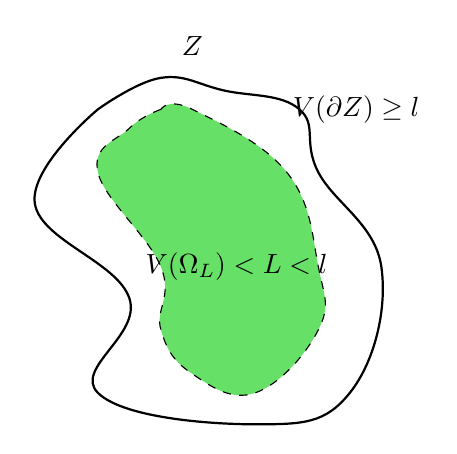
\begin{tikzpicture}[scale=0.8]
\draw [thick]  plot[smooth, tension=.7] coordinates {(-4,2.5) (-3,3) (-2,2.8) (-0.8,2.5) (-0.5,1.5) (0.5,0) (0,-2)(-1.5,-2.5) (-4,-2) (-3.5,-0.5) (-5,1) (-4,2.5)};
%Open set
\draw [dashed,fill=black!20!green!60!white]  plot[smooth, tension=.7] coordinates {(-3,2.5) (-3.5,2.2) (-4,1.5) (-3,0) (-3,-1) (-2.5,-1.7) (-1.5,-2) (-0.5,-1) (-0.5,0) (-1,1.5) (-2.5,2.5) (-3,2.5)};
%Nodes and names
\node at (-2.5,3.5) {$Z$};
\node at (0.1,2.5) {$V(\partial Z) \geq l$};
\node at (-1.8,0) {$V(\Omega_L) < L < l$};
\end{tikzpicture}
    \caption{Diagram showing that $\Omega_L \subset Z$, where $l = \sum_{k \in G}\min_{x \in \partial Z}\lambda_{min}(P_k)h_k\min_{\nu \in \{1,...,n\}}{\Bar{x}^2_{\nu}}$}
    \label{fig:set_omega_L}
\end{figure}
\end{frame}

\begin{frame}{Next Steps}
\begin{block}{}
Defining or estimating the set
    \begin{equation}
        C = \{x \in \Omega_L : \dot{V}(x) > 0\}
    \end{equation}
\end{block}
\begin{equation*}
        \forall x \in C, 
    x'\big[\sum_{j \in \mathcal{R}}\sum_{k \in G}h_kh_j(A'_jP_k + P_kA_j)+ \sum_{k \in G}\dot{h}_kP_k\big]x > 0
    \end{equation*}
Treating the two addends separately, we choose to
\begin{equation*}
x'\sum_{k \in G}\sum_{j \in \mathcal{R}}h_kh_j\big(A'_jP_k+P_kA_j\big)x < 0    
\end{equation*}
\end{frame}

\begin{frame}{Next Steps}
    To guarantee this, it is sufficient that
    \begin{equation} 
    \Upsilon_{kk} < 0, \forall k \in G
\end{equation}
\begin{equation} 
    \Upsilon_{kj} + \Upsilon_{jk} < 0, \forall k,j \in \mathcal{R}, j<k,
\end{equation}
where
\begin{equation}
    \Upsilon_{kj} = \begin{bmatrix}
    L_kA_j+A'_jL'_k & *\\
    P_k-L'_k+R_kA_j & -R_k-R'_k
    \end{bmatrix}
\end{equation}
\end{frame}

\begin{frame}{Next Steps}
\begin{itemize}
    \item Working on $x'\sum_{k \in G}\dot{h}_kP_kx > 0$
    \item Guarantee the $\sup_{x \in C}V(x)$ condition in the LMIs using the S-Procedure
\end{itemize}
    
\end{frame}

\section{UAV Application}

\begin{frame}{UAV Application}
    \begin{minipage}{0.35\textwidth}
    \begin{figure}
        \centering
        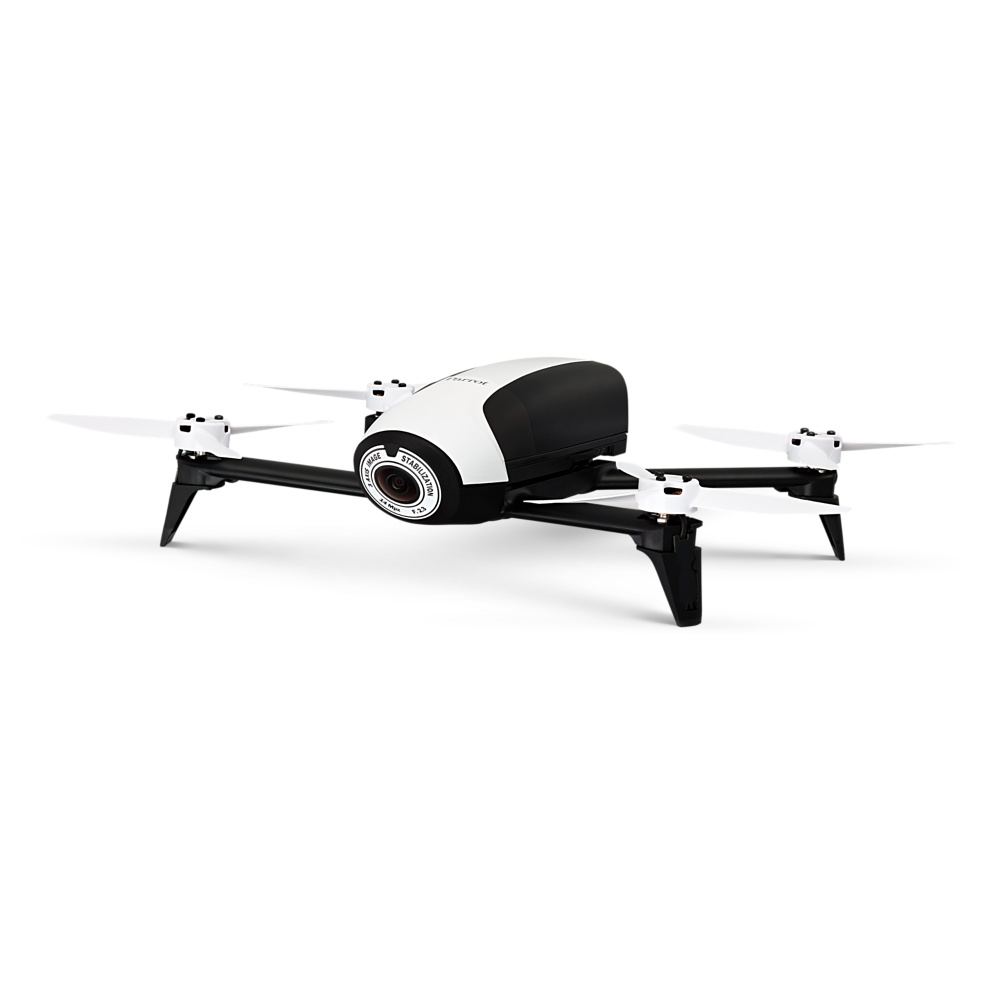
\includegraphics[scale=0.1]{figuras/new_bebop2_branco.jpg}
        \caption{Bebop 2}
        \label{fig:bebop2}
    \end{figure}
    \end{minipage} \hfill
    \begin{minipage}{0.55\textwidth}
    \begin{itemize}
        \item Unmanned Aerial Vehicles (UAVs) have been increasingly gaining popularity in robotics
        \item hover and vertical take off and landing 
        \item do not require a runway: more flexible
        \item highly complex, nonlinear, underactuated system
        \item Parrot Bebop 2: off the shelf, low price, internal hover controller, open source driver 
    \end{itemize}
    \end{minipage}
\end{frame}

\subsection{Implementation (BEBOP + ROS + VICON)}
\begin{frame}{Trajectory tracking implementation}
\begin{figure}
 \centering
    \begin{minipage}{0.45\textwidth}
        \centering
        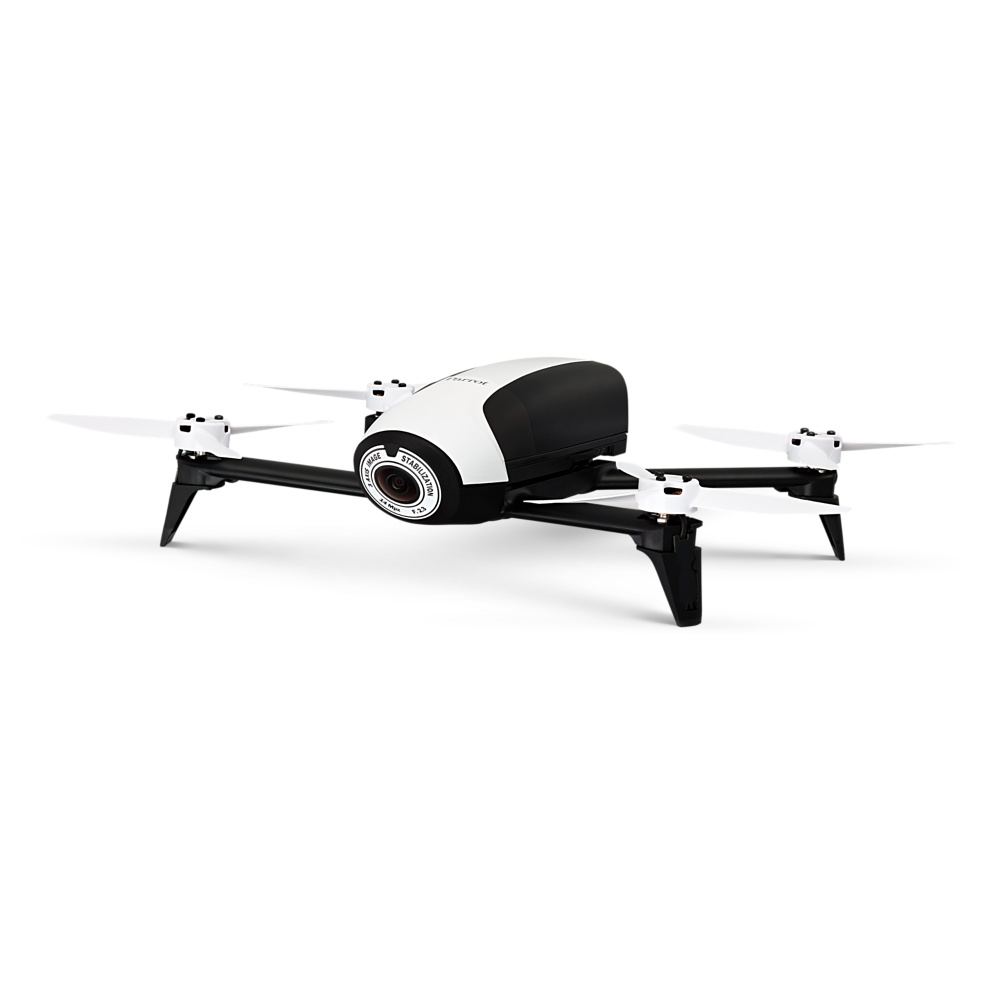
\includegraphics[scale=0.15]{figuras/new_bebop2_branco.jpg}
        \caption{Bebop 2}
    \end{minipage}\hfill
    \begin{minipage}{0.45\textwidth}
        \centering
        
\includegraphics[scale=0.3]{img/ros.png}
        \caption{Robot Operating System}
        
\includegraphics[scale=0.2]{figuras/vicon.jpg}
        \caption{Vicon Motion Capture Systems}
    \end{minipage}
    \end{figure}
\end{frame}

\begin{frame}{Closed loop}
Outdoor x Indoor experiments
    \begin{figure}[!htb]
	\centering
	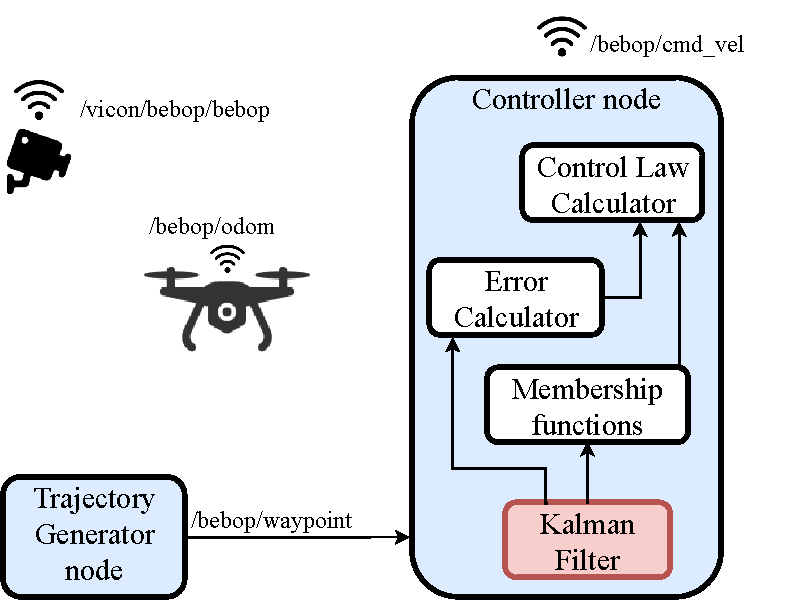
\includegraphics[scale=0.5]{figuras/control_scheme-Page-4.pdf}
	\caption{Block diagram showing the controller loop}
	\label{fig:control_scheme}
\end{figure}
\end{frame}



\subsection{Modeling (DINCON+others)}
%%%%%%%%%%%%%%%%%%%%%%%%%%%%%%%% FRAME %%%%%%%%%%%%%%%%%%%%%%%%%%%%%%%%

\begin{frame}{Quadcopter Model}
\begin{block}
	
Considering the the quadrotor's response to the input command vector  $u = \begin{bmatrix}
u_{\nu_x}&
u_{\nu_y}&
u_{\dot{z}}&
u_{\dot{\psi}}
\end{bmatrix}^T$, the dynamics can be modeled as the following linear system \autocite{VagoSantana2014a}

\begin{equation} \label{eq:Sant_lin}
\ddot{q}_b=\Gamma_A\dot{q}_b+\Gamma_Bu
\end{equation}
where $q_b = \begin{bmatrix}
x_b& 
{y}_b&
{z}_b&
{\psi}_b
\end{bmatrix}^T$ \begin{equation}
\Gamma_A=-\begin{bmatrix}
\gamma_2 & & & \\
&\gamma_4 & &\\
& &\gamma_6 &\\
& & &\gamma_8
\end{bmatrix}, ~\Gamma_B=\begin{bmatrix}
\gamma_1 & & & \\
&\gamma_3 & &\\
& &\gamma_5 &\\
& & &\gamma_7
\end{bmatrix}
\end{equation}

\end{block}

\end{frame}

%%%%%%%%%%%%%%%%%%%%%%%%%%%%%%%% FRAME %%%%%%%%%%%%%%%%%%%%%%%%%%%%%%%%
\begin{frame}
	For control purposes, it's more convenient to work with position and orientation with respect to a global stationary frame. \newline
	\newline
	Considering rotation only in the $z$ axis, we have
	\begin{equation} \label{eq:vel_trans}
	% ^{W}\dot{q} &= \prescript{W}{B}R ^{B}\dot{q}
	\dot{q} = R\dot{q_b} 
	\end{equation}
	where
	\begin{equation} \label{eq:R_matrix}
	R = \begin{bmatrix}
	\cos{\psi} & -\sin{\psi} & 0 & 0 \\
	\sin{\psi} & \cos{\psi} & 0 & 0 \\
	0 & 0 & 1 & 0 \\
	0 & 0 & 0 & 1
	\end{bmatrix}
	\end{equation}
\end{frame}

%%%%%%%%%%%%%%%%%%%%%%%%%%%%%%%% FRAME %%%%%%%%%%%%%%%%%%%%%%%%%%%%%%%%
\begin{frame}
	\begin{block}{Santana et. al. (2014) - Global Reference Frame}
			\begin{equation} \label{eq:robotic_dyn}
			\ddot{q}+NR^{T}\dot{q} = Mu, 
			\end{equation}
			\begin{eqnarray}
			M = \begin{bmatrix}
			\gamma_1\cos{\psi} & -\gamma_3\sin{\psi} & 0 & 0 \\
			\gamma_1\sin{\psi} & \gamma_3\cos{\psi} & 0 & 0 \\
			0 & 0 & \gamma_5 & 0 \\
			0 & 0 & 0 & \gamma_7
			\end{bmatrix} \\
			N =     \begin{bmatrix}
			\gamma_2\cos{\psi} & -\gamma_4\sin{\psi} & 0 & 0 \\
			\gamma_2\sin{\psi} & \gamma_4\cos{\psi} & 0 & 0 \\
			0 & 0 & \gamma_6 & 0 \\
			0 & 0 & 0 & \gamma_8
			\end{bmatrix}.
			\end{eqnarray}
	\end{block}	
\end{frame}

%%%%%%%%%%%%%%%%%%%%%%%%%%%%%%%% FRAME %%%%%%%%%%%%%%%%%%%%%%%%%%%%%%%%
% \begin{frame}{State Space Model}
% 	Let us define a state vector $\mathbf{\zeta} = \begin{bmatrix}
% 	\dot{q}^T & 
% 	q^T
% 	\end{bmatrix}^T = \begin{bmatrix}
% 	\dot{x} & 
% 	\dot{y}&
% 	\dot{z}&
% 	\dot{\psi} &
% 	{x} & {y} & {z} & {\psi}
% 	\end{bmatrix} ^T$. After some algebraic manipulation, one can obtain
% 	\begin{equation} \label{eq:SS}
% 	\dot{\mathbf{\zeta}} =   \begin{bmatrix}
% 	-NR^T & ~0\\
% 	~I  & ~0
% 	\end{bmatrix} \mathbf{\zeta} + \begin{bmatrix}
% 	M\\
% 	0
% 	\end{bmatrix}u
% 	\end{equation}
% 	where the input command vector is given by $u = \begin{bmatrix}
% 	u_{\nu_x}&
% 	u_{\nu_y}&
% 	u_{\dot{z}}&
% 	u_{\dot{\psi}}
% 	\end{bmatrix}^T$.
% \end{frame}
%%%%%%%%%%%%%%%%%%%%%%%%%%%%%%%% FRAME %%%%%%%%%%%%%%%%%%%%%%%%%%%%%%%%
\begin{frame}{Error Model}
\begin{block}{}
	Given a twice differentiable desired state trajectory $\zeta_d(t) = \begin{bmatrix}\dot{q}_d^T & q_d^T \end{bmatrix}^T$, let us define the tracking error $e = \mathbf{\zeta} - \mathbf{\zeta}_{d}$,
	\begin{equation} \label{eq:SS_error}
\dot{e} = \begin{bmatrix} 
-NR^T & 0 \\
I & 0
\end{bmatrix}e + \begin{bmatrix}
I\\
0
\end{bmatrix}\nu
\end{equation}
where $\nu = - \ddot{q}_d -NR^T\dot{q}_d + Mu$ is a virtual control input to the error system. The control input to be sent to the quadrotor system is given by
\begin{equation} \label{eq:real_control}
u = M^{-1} (\nu + \ddot{q}_d + NR^T\dot{q}_d)
% \nu = - \ddot{q}_d -NR^T\dot{q}_d + Mu
\end{equation} 
\end{block}
\end{frame}

\begin{frame}{System Analysis}

\begin{itemize}
    \item The origin is an unstable equilibrium point for system \eqref{eq:SS_error} and has an infinite number of equilibria located in $\{ e \in \mathbb{R}^8 :  e_1, e_2, e_3, e_4 = 0 \}$
    \item Hartman-Grobman Theorem does not apply (linearized system with non hyperbolic equilibria)
    \item To make the closed loop system have an unique equilibrium point at the origin, we modify \eqref{eq:real_control} 
\begin{equation}
    u = M^{-1} \left( \nu + \ddot{q}_d + NR^T\dot{q}_d -k(q-q_d) \right),
\end{equation} \label{eq:real_cont_new}
where $k$ is a positive scalar
\item \begin{equation}
    \Rightarrow \dot{e} = \begin{bmatrix}
-NR^T & -kI\\
I & 0
\end{bmatrix}e + \begin{bmatrix}
I\\
0
\end{bmatrix} \nu \label{eq:newclosedloop}
\end{equation}
\item We have not thoroughly studied the impact of this modification, but it seems to have increased the feasibility of the various LMI conditions we tested 
\end{itemize}
    
\end{frame}


\begin{frame}{LPV system}
	The error system is given by
	\begin{equation*} \label{eq:err_simple}
	\dot{e} =  A(\psi)e + B\nu
	\end{equation*} where
	
	\begin{equation*}
			A(\psi)=-\begin{bmatrix} \begin{array}{cccc|c}
				\gamma_{2}\cos^{2}(\psi) + \gamma_{4}\sin^{2}(\psi) &  \frac{\gamma_{4}-\gamma_{2}}{2}\sin(2\psi)&  &  & \multirow{4}{*}{0}\\
				\frac{\gamma_{2}-\gamma_{4}}{2}\sin(2\psi) & \gamma_{4}\cos^{2}(\psi) + \gamma_{2}\sin^{2}(\psi) &  &  &\\
				&  & \gamma_6 & &\\
				&  &  & \gamma_8& \\ \hline
				\multicolumn{3}{c}{-I} & & 0
				\end{array}
				\end{bmatrix}
	\end{equation*} and \begin{equation*}
		B = \begin{bmatrix}
				I\\
				0
			\end{bmatrix}\nu
			\end{equation*}
\end{frame}
%%%%%%%%%%%%%%%%%%%%%%%%%%%%%%%% FRAME %%%%%%%%%%%%%%%%%%%%%%%%%%%%%%%%
\begin{frame}{Modeling alternatives}
	Different choices of parameter vectors yield different representations. For example, choosing  
	\begin{equation} \label{eq:param_init}
	\rho(t) = \begin{bmatrix}
	\gamma_{2}\cos^{2}(\psi) + \gamma_{4}\sin^{2}(\psi) \\
	\frac{\gamma_{2}-\gamma_{4}}{2}\sin(2\psi)
	\end{bmatrix}
	\end{equation} 
	as the parameter vector, one can write 
	\begin{equation} \label{eq:err_LPV}
	\dot{e} =  (A_{0} + \sum_{i=1}^{2}A_{i}\rho_{i})e + B\nu
	\end{equation} 
	for some appropriate $A_i$, $i=0,\dots, 2$. The parameters bounds are given by 
	\begin{equation} \label{eq:param_init_bounds}
	\begin{aligned}
	\rho_{1} \in [\min(\gamma_{2},\gamma_{4}), ~\max(\gamma_{2},\gamma_{4})]\\
	\rho_{2} \in [-\frac{\gamma_{2}-\gamma_{4}}{2},~\frac{\gamma_{2}-\gamma_{4}}{2}].
	\end{aligned}
	\end{equation} 
\end{frame}
%%%%%%%%%%%%%%%%%%%%%%%%%%%%%%%% FRAME %%%%%%%%%%%%%%%%%%%%%%%%%%%%%%%%
\begin{frame}{Modeling alternatives}
	As an alternative we have 
	\begin{equation} 
	\rho(t) = \begin{bmatrix}
	\cos^{2}(\psi)\\
	\sin^{2}(\psi)\\
	\sin(2\psi)
	\end{bmatrix}
	\end{equation} with bounds  
	\begin{equation} \label{eq:param_final_bounds}
	\rho_{1},\rho_{2} \in [0, 1], ~\rho_{3} \in [-1,1]
	\end{equation} 
	which gives a representation of the form
	\begin{equation} \label{eq:err_LPV_final}
	\dot{e} =  (A_{0} + \sum_{i=1}^{3}A_{i}\rho_{i})e + B\nu
	\end{equation} 
\end{frame}

\begin{frame}{Modeling alternatives}
	Using the sector nonlinearity approach, the regular choice of premises would be
	\begin{subequations}
		\begin{eqnarray}
		z_1(t)&=&	\gamma_{2}\cos^{2}(\psi) + \gamma_{4}\sin^{2}(\psi)\\
		z_2(t)&=&\frac{\gamma_{2}-\gamma_{4}}{2}\sin(2\psi)
		\end{eqnarray}
	\end{subequations}
	However, choosing simpler premises 
	\begin{subequations}
		\begin{align}
		z_1(t)=\cos{\psi(t)} \\
		z_2(t)=\sin{\psi(t)}
		\end{align}
	\end{subequations} still gives an exact representation of the error system.
\end{frame}

% \begin{frame}{TS-fuzzy modeling}
% Continuing to build the TS-fuzzy model, we have 
% \begin{subequations} 
% 	\begin{align}
% 	z_1(t)&=\cos{\psi(t)}=(1)\omega_1^1+(-1)\omega_0^1 \\
% 	z_2(t)&=\sin{\psi(t)}=(1)\omega_1^2+(-1)\omega_0^2,
% 	\end{align}
% \end{subequations} where

% \begin{equation} 
% \sum_{i=0}^{1}\omega_{i}^{k} = 1 ~\forall k \in \{1,2\}.
% \end{equation}
% \end{frame}
%%%%%%%%%%%%%%%%%%%%%%%%%%%%%%%% FRAME %%%%%%%%%%%%%%%%%%%%%%%%%%%%%%%%
% \begin{frame}{TS modeling}
% 	We, then, find \begin{subequations} 
% 		\begin{align}
% 		w_0^1=\dfrac{z_1+1}{2},~ w_1^1=1-w_0^1\\
% 		w_0^2=\dfrac{z_2+1}{2},~ w_1^2=1-w_0^2.
% 		\end{align}
% 	\end{subequations}
% \end{frame}

\begin{frame}
	\begin{block}{TS-fuzzy model}
	The tracking error system can be thus represented as
	\begin{equation}
	\dot{e}(t) = \sum_{i=1}^{4}\sum_{j=1}^{4}h_i h_jA_{ij}e+B\nu =\sum_{i=1}^{4}\sum_{j=1}^{4}h_i h_j\begin{bmatrix}
	-N_iR_j^T & 0 \\
	I & 0
	\end{bmatrix}e+\begin{bmatrix}
	I\\
	0
	\end{bmatrix}\nu
	\end{equation} where $N_i,R_j$ are the matrices of the local models of the system and 
		\begin{equation} 
		\forall\, i\in\{1,\ldots, 4\},~~h_i(\psi) \geq 0 \text{~~and~~} \sum_{i=1}^{r}h_i(\psi)=1.
		\end{equation}
		\begin{equation}
		\begin{aligned}
		h_{1}(\psi)&=w_1^1(\psi)w_1^2(\psi),& h_{2}(\psi)&=w_1^1(\psi)w_0^2(\psi),\\
		h_{3}(\psi)&=w_0^1(\psi)w_1^2(\psi),& h_{4}(\psi)&=w_0^1(\psi)w_0^2(\psi). \\
			w_0^1&=\dfrac{\cos(\psi(t))+1}{2},~& w_1^1&=1-w_0^1\\
	w_0^2&=\dfrac{\sin(\psi(t))+1}{2},~& w_1^2&=1-w_0^2.
		\end{aligned}    
		\end{equation}

	\end{block}
\end{frame}

\begin{frame}{Models summary}
    \begin{table}[]
        \centering
        \begin{tabular}{c|c}
             $\#$ & Description \\ \hline
             1& 4 subsystems \\ \hline
             2& 16 subsystems\\ \hline
             3& 10 subsystems\\ \hline
             4& 8 subsystems\\ \hline
        \end{tabular}
        \caption{Summary of different modeling alternatives we developed}
        \label{tab:my_label}
    \end{table}
    \begin{block}{}
    All the models are equivalent to each other and exactly represent the nonlinear system. For proof, check \cite{Araujo2019}
    \end{block}
\end{frame}
    % \begin{frame}{TS modeling}
    % Rewriting the TS-fuzzy representation in a quasi LPV notation, we have
    % \begin{equation}
    % \dot{e}(t) = \mathcal{A}(\rho)e+B\nu
    % \end{equation}
    % with
    % \begin{eqnarray}
    % \mathcal{A}(\rho)& =& \sum_{i=1}^{9}\rho_i\mathcal{A}_i \nonumber\\&=&  \sum_{i=1}^{4}\sum_{j=1}^{4}h_i(\psi)h_j(\psi)\begin{bmatrix}
    % -N_iR_j^T & 0 \\
    % I & 0
    % \end{bmatrix}.
    % \end{eqnarray}
    % \end{frame}




\subsection{Control: SBAI, ICUAS, Output feedback results}
\begin{frame}{Controller Design via LMI}
	For all design procedures used, the controller is of the form
	\begin{equation}\label{FC}
	\nu=-\sum_{i=1}^{r}h_iK_ie
	\end{equation}
	where $r$ is the number of subsystems for each model
	
	\begin{block}{Remark}
	In implementation, the control signal sent to the system is 
	\begin{equation}
	    u = M^{-1} (-\sum_{i=1}^{r}h_iK_ie + \ddot{q}_d + NR^T\dot{q}_d) 
	\end{equation}
	\end{block}
\end{frame}


\begin{frame}{Stabilizing State Feedback}
\centering
$V(\mathbf{e}(t)):S \rightarrow \mathbb{R}^8, ~
V(\mathbf{e}(t))=\sum_{i=1}^{4}h_i\mathbf{e}(t)'\mathbf{P}_i\mathbf{e}(t), ~S \subset \mathbb{R}^8, ~\mathcal{R} = \{1,...,4\}$

\begin{theorem}
Let $\phi_{\rho}$ be known positive real numbers satisfying$|\dot{h}_{\rho}|\leq \phi_{\rho},\forall \rho\in \mathcal{R}$. If for a positive constant $\mu$, there exist matrices $\mathbf{ Z}\in \mathbb{R}^{8\times 8}$, $\mathbf{ Y}_{i}\in \mathbb{R}^{4\times 8}$, $\mathbf{X}=\mathbf{X}'\in \mathbb{R}^{8\times 8}$ and $\mathbf{Q}_{i}=\mathbf{Q}_{i}'\in \mathbb{R}^{8\times 8}$ satisfying \eqref{eqt31}-\eqref{eqt34}, then system \eqref{fuzzy}, with feedback $\nu = -\sum_{i=1}^{4}h_iK_ie$ and local gains $\mathbf{K}_{i}=\mathbf{Y}_{i}\mathbf Z^{-1}$, is asymptotically stable for any $\mathbf{e} \in \mathcal{D} :=\{\mathbf{e}\in S:|\dot{h}_{\rho}|\leq \phi_{\rho},~~\forall \rho\in\mathcal{R}\}$ .
\begin{align}
\label{eqt31} {\bf Q}_i\succ {\bf 0},&\quad \forall i\in \mathcal{R},\\[2mm]
\label{eqt32} {\bf Q}_\rho+{\bf X}\succeq{\bf 0},&\quad \forall \rho\in \mathcal{R},\\[2mm]
\label{eqt33} \Psi_{ii}\prec {\bf 0},&\quad \forall i\in \mathcal{R},\\[2mm]
\label{eqt34} \frac{1}{r-1}\Psi_{ii}+\Psi_{ij}+\Psi_{ji}\prec {\bf 0},&\quad \forall i,j\in \mathcal{R}, i<j
\end{align}
\end{theorem}
\end{frame}

\begin{frame}{}
    \begin{block}{Theorem (cont.)}
    where
\begin{align*}
\Psi_{ij}&=\begin{bmatrix}
{\bf \tilde{Q}}-{\bf A}_{ij}\mathbf{Z}-\mathbf{Z}'{\bf A}_{ij}'+{\bf B}\mathbf{Y}_i+\mathbf{Y}_i'{\bf B}' & \star \\
{\bf Q}_{i}-\mu\Bigl({\bf A}_{ij}\mathbf{Z}-{\bf B}\mathbf{Y}_i\Bigr)+\mathbf{Z}' & \mu\bigl(\mathbf{Z+Z}'\bigr)
\end{bmatrix},\\
{\bf \tilde{Q}}&=\sum^{4}_{\rho=1}\phi_\rho\left({\bf Q}_\rho+{\bf X}\right).
\end{align*}
    \end{block}
    
    \begin{proof}
    Check \cite{Araujo2019a}
    \end{proof}
\end{frame}

\begin{frame}{Experimental Results}
\begin{minipage}{0.45\textwidth}
        \centering
        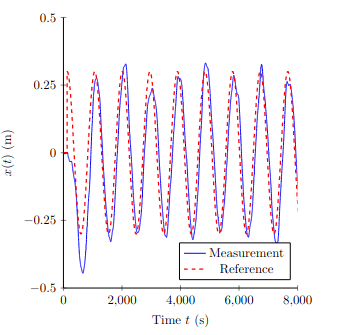
\includegraphics[scale=0.45]{img/sbaiX.png}
    \end{minipage}\hfill
    \begin{minipage}{0.45\textwidth}
        \centering
        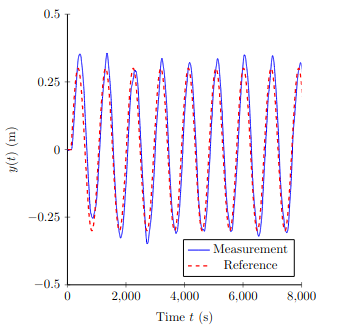
\includegraphics[scale=0.45]{img/sbaiY.png}
    \end{minipage}
    \begin{itemize}
        \item large initial error but the controller is able to correct it
        \item large error in the max and min values of the sinusoid caused by poor velocity estimation (will be discussed in the implementation section)
        \item otherwise, good tracking
    \end{itemize}
\end{frame}

\begin{frame}{Robust Stability - model uncertainty}
\begin{block}{Remark}
Results were accepted for conference, but the publication was cancelled due to the pandemic
\end{block}
Polytopic Uncertainty:
\begin{align}
\label{eq_fsysu}
\mathbf{\dot e} &= \sum_{k=1}^{2}\sum_{i=1}^{4}\sum_{j=1}^{4}\tilde{\alpha_k}h_ih_j(\mathbf{A}_{kij}-\mathbf{B}\mathbf{K}_i)\mathbf{e}+\mathbf{B}_{w}{\mathbf w}\\
\mathbf{y}&=\mathbf{C e}
\end{align}
${\tilde \alpha_k}$ model the uncertainty in parameters $\gamma_i, ~i=2,4,6,8$.  They satisfy the convex conditions ${\tilde \alpha_1}\geq 0$, ${\tilde \alpha_2}\geq 0$ and ${\tilde \alpha_1}+{\tilde \alpha_2}=1$. Input $w$ models the disturbance.
\begin{block}{}
Control design goal: find $K_i$
\end{block}
\end{frame}

\begin{frame}{Robust Stability} 
\begin{theorem}
If there exist a positive constant $\mu$, matrices ${\bf W} \in \mathbb{R}^{n_x\times n_x}$, ${\bf Y}_{i} \in \mathbb{R}^{n_u\times n_x}$ and $\mathbf{Q}_{i} \succ \mathbf{0} \in \mathbb{R}^{n_x\times n_x}$, $ ~\forall ~i \in \mathcal{R}$, satisfying
\begin{align}
\label{eq_lmis_teo}
% \begin{array}{c}
\Upsilon^{\ell}_{kii}\prec \mathbf{0}
\\[2mm]
\dfrac{2}{r-1}\Upsilon^{\ell}_{kii}+\Upsilon^{\ell}_{kij}+\Upsilon^{\ell}_{kji}\prec \mathbf{0},
% \end{array}
\end{align}
then, system \eqref{eq_fsysu}, with $\bf{w}(t)\neq \mathbf{0}$, local gains $\mathbf{K}_{i}=\mathbf{Y}_{i}\mathbf W^{-1}$, and $\displaystyle \phi=\max_{i \in \mathcal{R}} \{\phi_i\}$, is asymptotically stable for any solution contained in $\mathcal{D}=\left\{\mathbf{e}(t)\in \mathbb{R}^8:|\dot{h}_{i}|\leq \phi_{i},~~\forall i\in \mathcal{R}\right\}$,
\end{theorem}
\end{frame}

\begin{frame}{Robust Stability}
    \begin{block}{Theorem (cont.)}
    where $k\in\{1,2\}$, $i,j \in \mathcal{R}$, $i \not= j$, $\ell \in \{1,\ldots, \eta\}$
\begin{align}
\Upsilon^{\ell}_{kij}&= 
\left[\begin{array}{c}
\tilde{\mathbf{Q}}_\ell-{\bf A}_{kij}{\bf W}-{\bf W}'{\bf A}'_{kij}+{\bf B}{\bf Y}_{i}+{\bf Y}'_{i}{\bf B}'\\
{\bf Q}_{i}+{\bf W}'-\mu({\bf A}_{kij}{\bf W}-{\bf B}{\bf Y}_{i}) \end{array}\right.\\
& \hspace{5cm} \left.\begin{array}{c}
\star\\
\mu({\bf W}+{\bf W}')\end{array}\right]\\
\tilde{\mathbf{Q}}_\ell &= \tilde{\phi} \sum^{4}_{i=1}\mathbf{\tilde G}_{(i,\ell)} \mathbf{Q}_i
\end{align}
and $\mathbf{\tilde G}_{(i,\ell)}$ is the  element in the  $i^{th}$ row and $\ell^{th}$ column of matrix $\tilde{G}$
    \end{block}
\end{frame}

\begin{frame}{Matrix $\tilde{G}$}
    Define the set
\begin{equation}\label{eq_om}
\Omega:=\{v \in \mathbb{R}^4: -\phi_i\leq v_{i}\leq \phi_i, ~c'v=0\}
\end{equation}
where $c'=[1~~1~~1~~1]$ and $v_i$ is the $i^{th}$ coordinate of $v$. It represents the region of valid combinations of $\dot{h}_i$. The vertices of \eqref{eq_om} are organized in the following matrix\autocite{Mozelli2018}:
\begin{equation}
    \label{m_v}
\mathbf{\tilde G}:=\left[\begin{array}{cccc}
\mathbf{\tilde g}^1 & \mathbf{\tilde g}^2 &\ldots
& \mathbf{\tilde g}^{\eta}  \end{array}\right] \in \mathbb{R}^{4\times\eta}.
\end{equation}
where $\eta=\dfrac{4!}{2!2!}=6$.

\begin{itemize}
    \item Less conservative than assuming $|\dot{h}_i| = \phi_i$
\end{itemize}
\end{frame}

\begin{frame}{Results}
\begin{block}{}
There are both simulation and experimental results, but we decided to include only the simulation in the publication (timing reasons)
\end{block}
\begin{minipage}{0.45\textwidth}
        \centering
        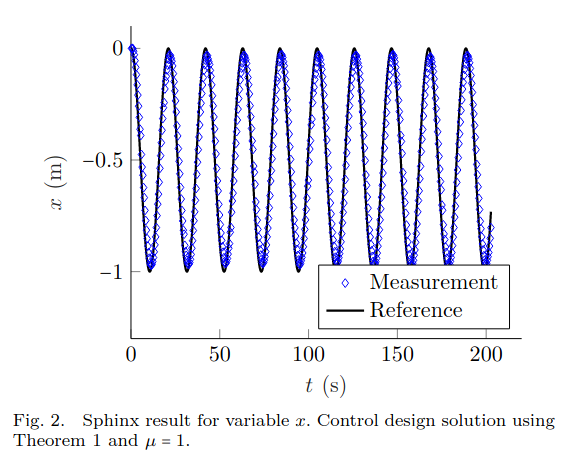
\includegraphics[scale=0.3]{img/icuas_x.png}
    \end{minipage}\hfill
    \begin{minipage}{0.45\textwidth}
        \centering
        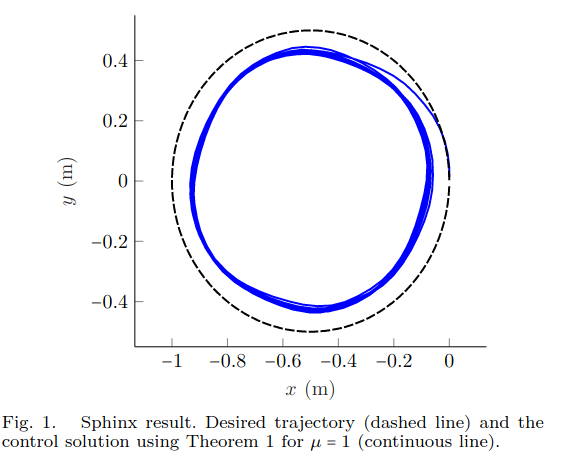
\includegraphics[scale=0.3]{img/icuas_xy.png}
    \end{minipage}
    \begin{itemize}
        \item Performance loss due to parameter uncertainty (steady state error)
        \item This uncertainty model is too conservative
    \end{itemize}
\end{frame}


\begin{frame}{$\mathcal{H}\infty$ performance}
\begin{theorem}
\label{teo2}
If there exist positive constants $\mu$ and $\gamma$, matrices ${\bf W} \in \mathbb{R}^{n_x\times n_x}$, ${\bf Y}_{i} \in \mathbb{R}^{n_u\times n_x}$ and $\mathbf{Q}_{i} \succ \mathbf{0} \in \mathbb{R}^{n_x\times n_x}$, $ ~\forall ~i \in \mathcal{R}$, satisfying 
\begin{align} \label{eq_lmis_teo2}
\Psi^{\ell}_{kii}\prec \mathbf{0}
\\[2mm]
\dfrac{2}{r-1}\Psi^{\ell}_{kii}+\Psi^{\ell}_{kij}+\Psi^{\ell}_{kji}\prec \mathbf{0}
\end{align}
Then, system \eqref{eq_fsysu} is stabilizable with local gains $\mathbf{K}_{i}=\mathbf{Y}_{i}\mathbf W^{-1}$, and $\mathcal{H}\infty$ guaranteed cost $\gamma$ for any solution $\mathbf{e}(t)$ contained in $\mathcal{D}=\left\{\mathbf{e}(t)\in \mathbb{R}^8:|\dot{h}_{i}|\leq \phi_{i},~~\forall i\in \mathcal{R}\right\}$,
\end{theorem}
\end{frame}

\begin{frame}{$\mathcal{H}\infty$ performance}
    \begin{block}{Theorem (cont.)}
    where $k\in\{1,2\}$, $i,j \in \mathcal{R}$, $i \not= j$, $\ell \in \{1,\ldots, \eta\}$, $\displaystyle \tilde{\phi}=\max_{i \in \mathcal{R}} \{\phi_i\}$
    \begin{align*}
\Psi^{\ell}_{kij}&= 
\left[\begin{array}{c}
\tilde{\mathbf{Q}}_\ell-{\bf A}_{kij}{\bf W}-{\bf W}'{\bf A}'_{kij}+{\bf B}{\bf Y}_{i}+{\bf Y}'_{i}{\bf B}'\\
{\bf Q}_{i}+{\bf W}'-\mu({\bf A}_{kij}{\bf W}-{\bf B}{\bf Y}_{i}) \\
-{\bf B}_{w}' \\
{\bf C}{\bf W} 
\end{array}\right.\\
& \hspace{3cm} \left.\begin{array}{ccc}
\star &  \star & \star\\
\mu({\bf W}+{\bf W}') & \star & \star\\
-\mu {\bf B}_{w}' & -\gamma^2 & \star\\
{\bf 0} & {\bf 0} & -{\bf I}
\end{array}\right]\\
\tilde{\mathbf{Q}}_\ell &= \tilde{\phi} \sum^{r}_{i=1}\mathbf{\tilde G}_{(i,\ell)} \mathbf{Q}_i
\end{align*}
with $\mathbf{\tilde G}$ defined in \eqref{m_v} and $\mathbf{\tilde G}_{(i,\ell)}$ the  element in its  $i^{th}$ row and $\ell^{th}$ column.
    \end{block}
\end{frame}

\begin{frame}{Results (simulation)}
\begin{block}{}
There are also experimental results (outdoor, wind measured)
\end{block}
\begin{minipage}{0.45\textwidth}
        \centering
        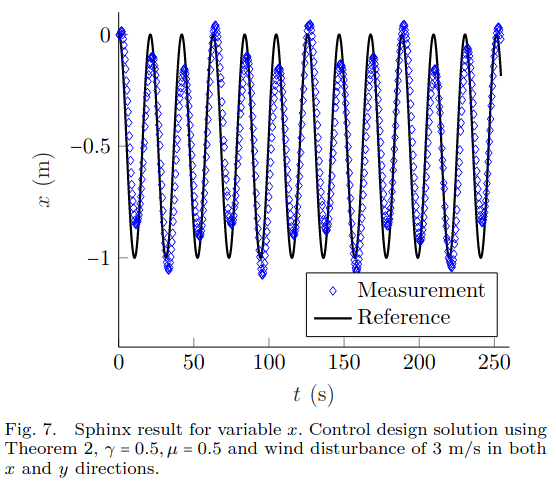
\includegraphics[scale=0.3]{img/icuas_x_teo2.png}
    \end{minipage}\hfill
    \begin{minipage}{0.45\textwidth}
        \centering
        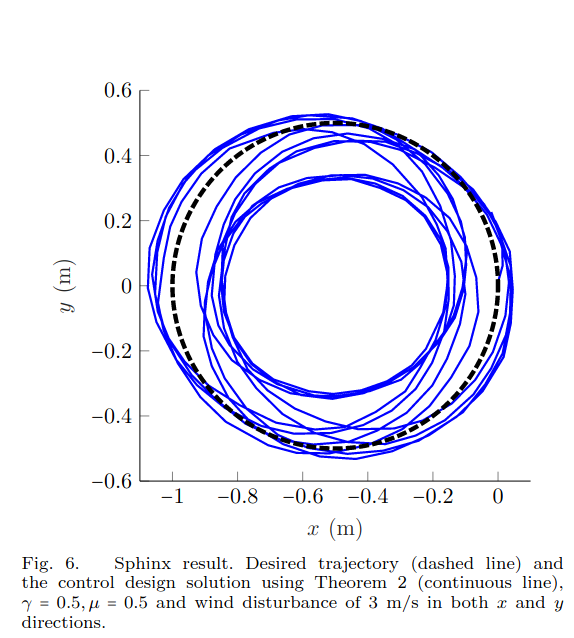
\includegraphics[scale=0.25]{img/icuas_xy_teo2.png}
    \end{minipage}
    \begin{itemize}
        \item Uncertainty model is too conservative and hinders the disturbance rejection
    \end{itemize}
\end{frame}

\begin{frame}{Bounds on control input}
Because of the application, we had to include bounds on the control input in all previous LMIs using the following lemma\autocite{Assuncao2007}
\begin{block}{Lemma}
Given positive constants $\vartheta_1$ and $\vartheta_2$, then the local gains $\mathbf{K}_{i}=\mathbf{Y}_{i}\mathbf W^{-1}$, $\forall\,i \in \mathcal{R}$, satisfies the condition $\mathbf{K}_{i}\mathbf{K}_{i}'<\vartheta_1I/\vartheta_2^2$ if the following LMIs hold:
\begin{equation}
    \label{umin}
\begin{gathered}
\left[ \begin{array}{cc} \vartheta_1 I & \mathbf{Y}_{i} \\
\mathbf{Y}_{i}'  & I \\
\end{array}\right] > 0   \\
{\mathbf Q}_i > \vartheta_2 I
\end{gathered}
\end{equation}
\end{block}
\begin{itemize}
    \item Control input is indirectly bounded by reducing the magnitude of entries of $\mathbf{K}_{i}$
    \item $\vartheta_1$ and $\vartheta_2$ are chosen appropriately 
\end{itemize}
\end{frame}

\begin{frame}{Static Output feedback}
\begin{itemize}
    \item Motivation: Not measuring all states + unsolved problem in the literature
    \item No feasibility
    \begin{itemize}
        \item various LMI conditions (based on the previous results and others from literature) $ \longrightarrow https://github.com/araujorayza/bebop\_control\_design$
        \item different model types
        
    \end{itemize}
    \item Controllability issues?
\end{itemize}
\end{frame}

\begin{frame}{Controllability Study}
\begin{itemize}
    \item Gap in literature
    \item Linearization $\longrightarrow$ no significant results
    \item Lyapunov based LMI analysis $\longrightarrow$ infeasibility not proven
\end{itemize}
\end{frame}

% \begin{frame}{Controllability Study for static output feedback}
% Closed loop of the system is of the form
% \begin{equation}
%     \dot{e}(t) = \begin{bmatrix}
%  \sum_{i=1}^{N}\rho_iL_i&-kI_4+\sum_{i=1}^{N}K_i\rho_i\\
%  I_4&0_4
% \end{bmatrix}e.
% \end{equation}
% \end{frame}

% \begin{frame}{Controller Design via LMI}
% 	The designed $Ks$ are 
% 	\begin{equation*}
% 	\begin{aligned}
% 	K_1 = \begin{bmatrix}
% 	1.03&   0.18&   0&    0&    0.45&    0&   0&    0\\
% 	0.18&    1.03&   0&   0&    0&    0.45&   0&   0\\
% 	0&    0&   -2.63&    0&    0&    0&    1.02&   0\\
% 	0&    0&   0&    0.89&   0&    0&   0&    1.02\\
% 	\end{bmatrix}\\
% 	K_2 = \begin{bmatrix}
% 	1.03&    0.18&    0&    0&    0.45&   0&    0&   0\\
% 	0.18&    1.03&   0&   0&   0&    0.45&    0&    0\\
% 	0&    0&   -2.63&    0&   0&    0&    1.02&   0\\
% 	0&    0&   0&    0.89&   0&    0&   0&    1.02\\
% 	\end{bmatrix}
% 	\end{aligned}
% 	\end{equation*}
	
% \end{frame}

% \begin{frame}{Controller Design via LMI}
% 	The designed $Ks$ are 
% 	\begin{equation*}
% 	\begin{aligned}
% 	K_3 = \begin{bmatrix}
% 	1.03&    0.18&   0&   0&    0.45&   0&   0&   0\\
% 	0.18&    1.03&   0&   0&   0&    0.45&    0&    0\\
% 	0&    0&   -2.63&    0&    0&    0&    1.02&   0\\
% 	0&    0&   0&    0.89&   0&    0&   0&    1.02\\
% 	\end{bmatrix}\\
% 	K_4 = \begin{bmatrix}
% 	1.03&   0.18&   0&   0&    0.45&    0&   0&   0\\
% 	0.18&    1.03&   0&   0&    0&    0.45&    0&    0\\
% 	0&    0&   -2.63&    0&    0&    0&    1.02&   0\\
% 	0&    0&   0&    0.89&   0&    0&   0&    1.02\\
% 	\end{bmatrix}
% 	\end{aligned}
% 	\end{equation*}
	
% \end{frame}



\section{Publications}
\begin{frame}{Publications (Journals)}
	\begin{itemize}
		\item ELIAS, LEANDRO JOSE ; FARIA, FLAVIO ANDRADE ; ARAUJO, R. ; MAGOSSI, RAFAEL ; OLIVEIRA, VILMA ALVES . \textbf{Robust static output feedback H control for uncertain Takagi-Sugeno fuzzy systems}. IEEE Transactions on Fuzzy Systems, v. 1, p. 1-1, 2022. 
		\item Leandro J. Elias, Flávio A. Faria, Rayza Araujo, Vilma A. Oliveira. \textbf{Stability analysis of Takagi–Sugeno systems using a switched fuzzy Lyapunov function}. Information Sciences, Volume 543, 2021, Pages 43-57, ISSN 0020-0255.
		
		\item ELIAS, LEANDRO J. ; FARIA, FLÁVIO A. ; ARAUJO, RAYZA ; OLIVEIRA, VILMA A. . \textbf{Stability conditions of TS fuzzy systems with switched polynomial Lyapunov functions.} IFAC-PAPERSONLINE, v. 53, p. 6352-6357, 2020.
	\end{itemize}
\end{frame}

\begin{frame}{Publications}
	\begin{itemize}
		\item F. Q. MAGOSSI, RAFAEL; ARAÚJO, RAYZA ; J. ELIAS, LEANDRO ; A. FARIA, FLÁVIO ; A. OLIVEIRA, VILMA . \textbf{Projeto de controlador de ordem fixa via LMI com limitação da norma H-infinito e garantias de margens de estabilidade.} In: Congresso Brasileiro de Automática 2020, 2020, Porto Alegre. Anais do Congresso Brasileiro de Automática 2020, 2020. 
		
		\item ARAUJO, R. ; ELIAS, L. J. ; FARIA, F. A. ; OLIVEIRA, V. A. . \textbf{On the selection of membership functions of TS fuzzy models for a commercial quadrotor.} In: XIV Conferência Brasileira de Dinâmica, Controle e Aplicações, 2019, São Carlos. Anais da XIV Conferência Brasileira de Dinâmica, Controle e Aplicações, 2019. p. 1-7. 
	\end{itemize}
\end{frame}

\begin{frame}{Publications}
	\begin{itemize}
		\item ARAUJO, R. ; FARIA, F. A. ; ELIAS, L. J. ; OLIVEIRA, V. A. . \textbf{Trajectory Tracking for the Bebop Parrot quadrotor using Takagi-Sugeno fuzzy models.} In: XIV Simpósio Brasileiro de Automação Inteligente, 2019, Ouro Preto. Anais do XIV Simpósio Brasileiro de Automação Inteligente. Campinas: SBA, 2019. p. 1-6. 
		
		\item FARIA, FLAVIO A. ; ELIAS, LEANDRO J. ; ARAUJO, RAYZA ; OLIVEIRA, VILMA A. . \textbf{Less conservative state feedback design conditions for switched Takagi-Sugeno fuzzy systems. }In: 2019 18th European Control Conference (ECC), 2019, Naples. 2019 18th European Control Conference (ECC), 2019. p. 3698. 
		
		\item MAGOSSI, R. F. Q.; BEZERRA, R. A. ; LEME, P. V. ; OLIVEIRA, V. A. . \textbf{PID Controller Design Based On H$\infty$ Performance.} In: XIII Simpósio Brasileiro de Automação Inteligente, 2017, Porto Alegre. XIII Simpósio Brasileiro de Automação Inteligente, 2017. p. 1814-1820.
	\end{itemize}
\end{frame}

\begin{frame}{Unpublished results}
	\begin{itemize}
		\item Survey on Gain Scheduling
		
		\item Control law modification
		
		\item "Robust Trajectory Tracking for the Bebop Parrot quadrotor using fuzzy
PDC controllers" 
\begin{itemize}
    \item accepted, but unpublished because of the pandemic
    \item there is still experiment data to be added, so it can easily be expanded
\end{itemize}
		\item LPV and T-S Fuzzy relationship analysis*
		
		\item LaSalle extension for T-S Fuzzy systems*
		
		\item Static Output feedback design and controllability for quadrotor*
	\end{itemize}
	\vspace{2cm}
	*still working on the results
\end{frame}

